\newpage
\chapter{СРАВНИТЕЛЬНЫЙ АНАЛИЗ РАЗРАБОТАННЫХ АЛГОРИТМОВ}
\label{chap:ExpResults}

\section{Вводные замечания}
\label{chap:ExpResults:Intro}

В разделах~\ref{chap:SIG} и~\ref{chap:CNM} данной работы было приведено описание двух новых алгоритмов обработки видеинформации в рамках системы распределенного видеокодирования. Следует отметить, что задача сравнительной оценки эффективности данных алгоритмов является сложной задачей ввиду того, что в открытом доступе нет исходного кода распределенного видеокодека, который можно было бы принять за <<эталонный>>. Кодек, разработанный в рамках проекта  DISCOVER~\cite{Artigas2007}, не предоставляет возможности внесения изменений, т.~к. распространяется только в виде бинарного исполняемого файла. Кроме проекта DISCOVER существует три открытых исследовательских проекта, посвященных распределенному кодированию.

\begin{itemize}
    \item Проект BLAST-DVC (BitpLAne SelecTive Distributed Video Coding)~\cite{5074834}. Основная цель данного проекта заключается в разработке распределенного видеокодека, расширяющего модель DISCOVER возможностью оценки важности битовых плоскостей с точки зрения кривой <<скорость-искажение>>. В схеме BLAST-DVC декодер запрашивает у кодера не все битовые плоскости квантованных спектральных коэффициентов, начиная с наиболее значимого спектрального коэффициента, а только те, которые ему необходимо восстановить для обеспечения заданного качества восстановления. Результат проекта доступен в виде исполняемого файла.
    
    \item Проект OpenDVC~\cite{6471251}. В результате данного проекта предполагалась разработка открытой реализации распределенного видеокодека. В качестве базовых модулей использовались алгоритмы, схожие с алгоритмами из базовой модели DISCOVER. Однако цель данного проекта не была достигнута, в настоящее время проект больше не развивается, хотя доступны исходные коды промежуточных версий кодека. Следует отметить, что исходный код OpenDVC характеризуются наличием большого числа ошибок и неточностей. Этот факт, а также отсутствие какой-либо документации и научных статей, описывающих OpenDVC, не позволяют использовать результаты данного проекта в качестве эталонного кодека.
    
    \item Проект Stanford DVC~\cite{Varodayan:2008:WCV:1379459.1379595}. В данном проекте основное внимание уделялось разработке адаптивных по скорости помехоустойчивых кодов для распределенного кодирования видеоданных, в частности, LPDCA кодов. Результаты данного проекта используются в кодеках DISCOVER, OpenDVC и BLAST-DVC для блока помехоустойчивого кодирования.
\end{itemize}

Таким образом, можно сделать вывод о том, что в настоящее время не существует открытой завершенной реализации распределенного видеокодека, и для проведения сравнительной экспериментальной оценки требуется в первую очередь разработать эталонный программный комплекс, реализующий основные концепции распределенного видеокодирования и позволяющий исследовать различные алгоритмы обработки видеоинформации в рамках данного подхода. В связи с этим настоящий раздел начинается с описания ключевых алгоритмов, особенностей и возможностей разработанной программной модели распределенного видеокодека. Далее приводится описание проведенных экспериментов для демонстрации выигрыша от применения разработанных алгоритмов и основные практические результаты, полученные с использованием данной программной модели. Перед тем, как переходить к описанию программного комплекса, введем в рассмотрение основные критерии сравнения алгоритмов сжатия видеоинформации, а также опишем тестовое множество видеопоследовательностей, которое будет использоваться в дальнейшем при сравнении.

\section{Критерии сравнения алгоритмов сжатия видеоданных}
\label{chap:ExpResults:Criteria}

Для количественного оценивания искажений, внесенных в изображение в результате обработки, как правило, используют критерий PSNR (пиковое отношение сигнал-шум), рассчитанный по яркостной компоненте. Для 8-битных компонент $\mathbf{Y}$ и $\widehat{\mathbf{Y}}$ значение PSNR рассчитывается как
\begin{equation}
\mathrm{PSNR}(\mathbf{Y},\widehat{\mathbf{Y}}) = 10 * \log_{10} \frac{255^2}{\mathrm{MSE}(\mathbf{Y},\widehat{\mathbf{Y}})},
\end{equation}
где $\mathrm{MSE}(\cdot,\cdot)$~--~среднеквадратичное отклонение, определяемое как
\begin{equation}
\mathrm{MSE}(\mathbf{Y},\widehat{\mathbf{Y}}) = \frac{1}{w*h} \sum\limits_{i=1}^{h}\sum\limits_{j=1}^{w} \left(\mathbf{Y}[i,j]-\widehat{\mathbf{Y}}[i,j]\right)^2,
\end{equation}
$w$, $h$~--~количество столбцов и строк в компоненте соответственно.

Чем выше значение PSNR, тем больше похожи компоненты $\mathbf{Y}$ и $\widehat{\mathbf{Y}}$. Считается, что $\mathrm{PSNR}>40$ соответствует очень высокой схожести изображений, когда искажения почти неразличимы человеческим глазом. Следует отметить, что в настоящее время существует большое число работ, в которых показывается, что данный критерий во многих случаях слабо коррелирует с человеческим восприятием искажений. В связи с этим ведутся активные исследования в области разработки новых критериев, например SSIM, MS-SSIM. Однако, несмотря на критику, PSNR до сих пор является наиболее распространенным критерием в различных прикладных задачах цифровой обработки изображений. По этой причине в данной диссертационной работе будут использоваться критерии основанные в первую очередь на расчете значения PSNR между парой изображений (компонент изображений).

В рамках задачи сравнительной оценки алгоритмов временной интерполяции, как правило, используются следующие критерии:
\begin{itemize}
    \item графики покадрового значения PSNR;
    \item среднее значение PSNR, расчитанное по всем интерполированным кадрам.
\end{itemize}

Графики покадрового PSNR позволяют выделить кадры, характеризующиеся, например, низким качеством интерполяции. Данные кадры могут быть использованы для определения узких мест алгоритма и повышения качества интерполяции в целом.

Среднее значение PSNR позволяет судить об эффективности алгоритма в целом. Именно этот критерий является наиболее распространенным при принятии решении о том, какой алгоритм интерполяции лучше.

Основным методом сравнения алгоритмов сжатия видеоданных является анализ кривых <<скорость-искажение>>, показывающих для заданной битовой скорости среднее значение PSNR для восстановленных кадров, а также оценка численных критериев, основанных на них. Наиболее распространенным методом сравнения кривых <<скорость-искажение>> является анализ критерия Бьёнтегаарда~\cite{Bjontegaard2001}, позволяющего оценить численно расстояние между двумя кривыми. Расстояние может выражаться в децибелах (BD-PSNR), показывая среднее различие по PSNR, или в процентах (BD-RATE), показывая относительное различие в битовой скорости. В настоящее время критерий BD-RATE является общепринятым при сравнительном анализе алгоритмов сжатия в процессе разработки новых стандартов кодирования видеоинформации.

\section{Формирование тестового множества видеопоследовательностей}
\label{chap:ExpResults:SchemeofExperiment:TestSet}

Кодек DISCOVER поддерживает обработку видеопоследовательностей с разрешением CIF ($352\times288$) или QCIF ($176\times144$) в формате YUV420, т.~е. каждый кадр представлен одной яркостной составляющей Y и двумя хроматическими составляющими U, V. Сжатию подвергается только компонента Y.

Стандартное тестовое множество кодека DISCOVER включает в себя четыре последовательности с разрешением QCIF~\cite{5134}.
\begin{itemize}
    \item Coastguard. В последовательности преобладает горизонтальное равномерное смещение. Кадры характеризуются большим количеством незначимых для визуального восприятия текстурных элементов.
    \item Foreman. Первая половина последовательности содержит изображение объекта, незначительно перемещающегося в центре сцены. Перемещение характеризуется наличием существенных деформаций формы объекта. Во второй половине происходит быстрое горизонтальное смещение с изображения объекта на статичную сцену.
    \item Hall. Представляет собой видео, снятое с камеры видеонаблюдения, установленной в коридоре. Характеризуется наличием заметных шумов, отсутствием смещения камеры и небольшим движением в центре сцены на протяжении почти всей последовательности.
    \item Soccer. Последовательность характеризуется быстрым и сложным движением небольшого числа объектов.
\end{itemize}

Т.~к. видео с разрешением QCIF в настоящее время можно считать мало репрезентативным, в данной диссертационной работе предлагается при проведении экспериментов использовать данные последовательности c максимально поддерживаемым кодеком DISCOVER разрешением~--~CIF. Кроме того, предлагается расширить тестовое множество, добавив в него одну последовательность с быстрым движением~--~Football.

\section{Описание разработанной программной модели распределенного видеокодека}
\label{chap:ExpResults:CodecModel}

В основе разработанной программной модели распределенного видеокодека лежит архитектура Стэнфорд, т.~е. в качестве единицы обрабатываемых кодеком Слепяна-Вулфа данных выступает кадр целиком. Модель кодека представляет собой реконфигурируемый программный комплекс, предоставляющий возможность замены модулей при условии сохранения интерфейса взаимодействия отдельных блоков системы. В качестве базовой реализации для всех модулей применяются методы, основанные на подходах из базовой модели DISCOVER. Однако, в силу того что в открытой литературе нет достаточно подробного описания всех особенностей реализации данных алгоритмов в DISCOVER (более того, в некоторых статьях дано различное описание одних и тех же блоков), верификация разработанной программной модели не представляется возможной. Как будет продемонстрировано далее, результаты полученные с использованием разработанного программного комплекса не совпадают с результатами DISCOVER. Тем не менее адекватность применения разработанного программного комплекса для решения задачи оценки эффективности различных алгоритмов распределенного видеокодирования является обоснованной, в силу того, что производительность данной модели с точки зрения критерия <<скорость-искажение>> сравнима (или даже превосходит) с производительностью кодека на основе проекта DISCOVER.

Приведем краткое описание процесса сжатия видеоинформации в разработанной программной модели распределенного видеокодека. Видеопоследовательность, представляющая собой последовательность кадров в формате YUV $4$:$2$:$0$, разбивается на две подпоследовательности:
\begin{itemize}
  \item базовые (ключевые, опорные) кадры;
  \item промежуточные кадры.
\end{itemize}

В рамках разработанной программной модели поддерживается только обработка группы кадров длины $2$ (GOP=2). Т.~е. если нумерация кадров в последовательности начинается с~$1$, то каждый второй кадр является промежуточным.

\subsection{Обработка базовых кадров}
\label{chap:ExpResults:CodecModel:KeyFrames}

Для обработки базовых кадров в разработанном кодеке используется эталонная реализация стандарта H.264/AVC~--~JM 9.5~\cite{h264jm}. Выбор версии 9.5 обусловлен тем фактом, что именно данная версия программного кода используется в кодеке DISCOVER. Обработка осуществляется в режиме INTRA, т.~е. без устранения межкадровой избыточности. 

Возможна обработка $8$-битных видеопоследовательностей двух возможных разрешений: CIF ($352\times288$) и QCIF ($176\times144$).

Для обеспечения воспроизводимости полученных результатов, параметры кодека базовых кадров приведены в приложении~\ref{AppB}.

По аналогии с кодеком DISCOVER в разработанном программном комплексе зафиксировано $8$ возможных уровней качества сжатия, параметры квантования ($QP$) для каждой тестовой последовательности для каждого уровня качества заданы в соответствии с таблицей~\ref{tab:IntraQP}. Данные параметры используются для всех тестовых разрешений. Следует отметить, что в кодеке DISCOVER указаны значения шагов квантования для последовательностей Coastguard, Foreman, Hall и Soccer. Для последовательности Football предлагается использовать те же параметры, что и для Soccer.

\begin{table}[!h]
    \caption{Параметры квантования ($QP$) ключевых кадров для тестовых последовательностей}
    \begin{center}
        \label{tab:IntraQP}
        \begin{tabular}{|c|c|c|c|c|c|c|c|c|}
            \hline
            \backslashbox{Последовательность}{Уровень качества} & $1$ & $2$ & $3$ & $4$ & $5$ & $6$ & $7$ & $8$ \\
            \hline
            Coastguard & $38$ & $37$ & $37$ & $34$ & $33$ & $31$ & $30$ & $26$ \\
            \hline
            Foreman & $40$ & $39$ & $38$ & $34$ & $34$ & $32$ & $29$ & $25$ \\
            \hline
            Hall & $37$ & $36$ & $36$ & $33$ & $33$ & $31$ & $29$ & $24$ \\
            \hline
            Soccer & $44$ & $43$ & $41$ & $36$ & $36$ & $34$ & $31$ & $25$ \\
            \hline
            Football & $44$ & $43$ & $41$ & $36$ & $36$ & $34$ & $31$ & $25$ \\
            \hline
        \end{tabular}
    \end{center}
\end{table}

\subsection{Кодер промежуточных кадров}
\label{chap:ExpResults:CodecModel:WZFramesEncoder}

Каждый промежуточный кадр кодируется независимо от остальных, обрабатывается только яркостная составляющая. На стороне кодера выполняются следующие действия:
\begin{enumerate}
  \item\label{DVCEncoder:DCT} \textbf{Блоковое дискретное косинусное преобразование}. Кадр разбивается на непересекающиеся блоки размером~$4\times4$ пикселя. Каждый блок~$\mathbf{B}^{(p)}$, где $p$~--~индекс блока, подвергается целочисленному преобразованию, определяемому как:
  \begin{equation*}
  \mathbf{T}^{(p)} = (\mathbf{C} \mathbf{B}^{(p)} \mathbf{C}^T) \circ \mathbf{E},
  \end{equation*}
  где $\circ$~--~поэлементное умножение матриц и
  \begin{equation*}
  \mathbf{C} = \begin{bmatrix}
  1 & 1 & 1 & 1 \\
  2 & 1 & -1 & -1 \\
  1 & -1 & -1 & 1 \\
  1 & -2 & 2 & -1
  \end{bmatrix},
  \end{equation*}
  \begin{equation*}
  \mathbf{E} = \begin{bmatrix}
  a^2 & \frac{ab}{2} & a^2 & \frac{ab}{2} \\
  \frac{ab}{2} & \frac{b^2}{4} & \frac{ab}{2} & \frac{b^2}{4} \\
  a^2 & \frac{ab}{2} & a^2 & \frac{ab}{2} \\
  \frac{ab}{2} & \frac{b^2}{4} & \frac{ab}{2} & \frac{b^2}{4}
  \end{bmatrix},
  \end{equation*}
  \begin{equation*}
  a = 0.5,
  \end{equation*}
  \begin{equation*}
  b = \sqrt{\frac{2}{5}}.
  \end{equation*}
  Полученные коэффициенты далее собираются в $16$ групп:
  \begin{equation*}
  \mathbf{g}^{(k,l)} = \left(\mathbf{T}^{(p)}[k,l]\right), p=1,2,\ldots,\frac{wh}{16},
  \end{equation*}
  где $\mathbf{T}^{(p)}[k,l]$~--~элемент, находящийся на позиции $(k,l)$ в блоке спектральных коэффициентов $\mathbf{T}^{(p)}$, $w$ и $h$~--~ ширина и высота кадра соответственно.
  
  Таким образом, для кадра с разрешением CIF в каждой группе содержится $6336$ спектральных коэффициентов, а для QICF~--~$1584$ спектральных коэффициента.
  
  \item\label{DVCEncoder:Quantization} \textbf{Квантование}. Полученные спектральные коэффициенты  далее подвергаются скалярному квантованию. Шаг квантования рассчитывается для каждой группы исходя из заранее заданной матрицы квантования~(\ref{eq:QuantizationMatrices}) для данного уровня качества и динамического диапазона данных.
  \begin{gather}
  \mathbf{Q}^{(1)} =
  \begin{bmatrix}
  16 & 8 & 0 & 0 \\
  8 & 0 & 0 & 0 \\
  0 & 0 & 0 & 0 \\
  0 & 0 & 0 & 0
  \end{bmatrix}
  \mathbf{Q}^{(2)} =
  \begin{bmatrix}
  32 & 8 & 0 & 0 \\
  8 & 0 & 0 & 0 \\
  0 & 0 & 0 & 0 \\
  0 & 0 & 0 & 0
  \end{bmatrix}
  \mathbf{Q}^{(3)} =
  \begin{bmatrix}
  32 & 8 & 4 & 0 \\
  8 & 4 & 0 & 0 \\
  4 & 0 & 0 & 0 \\
  0 & 0 & 0 & 0
  \end{bmatrix}
  \nonumber\\
  \mathbf{Q}^{(4)} =
  \begin{bmatrix}
  32 & 16 & 8 & 4 \\
  16 & 8 & 4 & 0 \\
  8 & 4 & 0 & 0 \\
  4 & 0 & 0 & 0
  \end{bmatrix}
  \mathbf{Q}^{(5)} =
  \begin{bmatrix}
  32 & 16 & 8 & 4 \\
  16 & 8 & 4 & 4 \\
  8 & 4 & 4 & 0 \\
  4 & 4 & 0 & 0
  \end{bmatrix}
  \mathbf{Q}^{(6)} =
  \begin{bmatrix}
  64 & 16 & 8 & 8 \\
  16 & 8 & 8 & 4 \\
  8 & 8 & 4 & 4 \\
  8 & 4 & 4 & 0
  \end{bmatrix}
  \nonumber \\
  \mathbf{Q}^{(7)} =
  \begin{bmatrix}
  64 & 32 & 16 & 8 \\
  32 & 16 & 8 & 4 \\
  16 & 8 & 4 & 0 \\
  8 & 4 & 0 & 0
  \end{bmatrix}
  \mathbf{Q}^{(8)} =
  \begin{bmatrix}
  128 & 64 & 32 & 16 \\
  64 & 32& 16 & 8 \\
  32 & 16 & 8 & 4 \\
  16 & 8 & 4 & 0
  \end{bmatrix}
  \label{eq:QuantizationMatrices}
  \end{gather}
  
  Коэффициенты DC подвергаются равномерному скалярному квантованию в диапазоне $[0,2^{11})$ (для $8$-битного входа) с числом квантов, равным левому верхнему значению в соответствующей матрице квантования~\ref{eq:QuantizationMatrices}.
  
  Для AC коэффициентов применяется скалярное квантование с удвоенным интервалом вокруг нуля. Шаг квантования в группе $(i,j)$ для уровня качества $q$ определяется как
  \begin{equation*}
  \Delta^{(k,l)} = \left\lceil\frac{2 m_{k,l}}{\mathbf{Q}^{(q)}[k,l]}\right\rceil,\text{ если $\mathbf{Q}^{(q)}[k,l] \neq 0$}.
  \end{equation*}
  где $m_{k,l}$~--~максимальное по модулю значение в группе $(k,l)$. Если $\mathbf{Q}^{(q)}[k,l] = 0$, то спектральные коэффициента в группе не квантуются и данные о них далее на стороне кодера не обрабатываются.
  
  Таким образом, индексы квантов $q_i^{(k,l)}$ в группе $(k,l)$ после квантования занимают $\log_2{\left(\mathbf{Q}^{(q)}[k,l]\right)}$ бит.
  
  \item\label{DVCEncoder:BitplaneExtraction} \textbf{Формирование битовых плоскостей}. Индексы квантов~$q_{(k)}^{(i,j)}$ разбиваются на битовые плоскости таким образом, что биты одной значимости попадают в одну плоскость. Обозначим $j$-й по значимости бит спектрального коэффициента, находящегося на позиции $i$ в группе $(k,l)$, через $b_j^{(k,l,i)}$. Для определенности будем считать, что наиболее значимая битовая плоскость имеет индекс $1$.
  
  \item \textbf{Помехоустойчивое кодирование}. Биты индексов квантов кодируются LDPCA кодом, начиная с наиболее значимой битовой плоскости в позиции наиболее значимого спектрального коэффициента. Накопленный синдром сохраняется в промежуточном буфере.
\end{enumerate}

Таким образом, кодер промежуточных кадров должен передать декодеру следующую информацию.
\begin{itemize}
  \item Один раз для всей последовательности: размеры кадра, параметр качества.
  \item Для каждого кадра: динамический диапазон данных в каждой группе спектральных коэффициентов, кроме DC.
\end{itemize}

Следует отметить, что т.~к. в данной работе не проводились исследования с целью снижения количества запросов декодером проверочных бит, в разработанном кодеке не используется модуль управления битовой скоростью на стороне кодера, присутствующий в схеме DISCOVER.

\subsection{Декодер промежуточных кадров}
\label{chap:ExpResults:CodecModel:WZFramesDecoder}

В разработанном программном комплексе на стороне декодера в процессе восстановления промежуточных кадров выполняются следующие действия.
\begin{enumerate}
  \item \textbf{Генерация дополнительной информации}. Алгоритм генерации дополнительной информации включает в себя следующие действия.
  \begin{enumerate}
    \item Выполняется процедура предсказания промежуточного кадра c использованием алгоритма временной интерполяции кадров, описанного в подразделе~\ref{chap:SIG:ReferenceAlgo}.
    \item К аппроксимирующему кадру применяется блоковое дискретное косинусное преобразование (аналогично шагу~\ref{DVCEncoder:DCT} на кодере).
    \item Квантование спектральных коэффициентов (аналогично шагу~\ref{DVCEncoder:Quantization} на кодере). Следует отметить, что т.~к. после дискретного косинусного преобразования спектральные коэффициенты могут выйти за границы динамического диапазона, рассчитанного на кодере, перед квантованием выполняется клипирование данных:
    \begin{equation*}
    \hat{g}^{k,l}_i = \begin{cases}
    & m_{k,l}\text{, eсли $\hat{g}^{k,l}_i \geq m_{k,l}$ } \\
    & -m_{k,l}\text{, eсли $\hat{g}^{k,l}_i < -m_{k,l}$ } \\
    & \hat{g}^{k,l}_i\text{, иначе}
    \end{cases},
    \end{equation*}
    где $m_{k,l}$~--~число, определяющее динамический диапазон данных (получено от кодера), $\hat{g}^{k,l}_i$~--~оцененный декодером спектральный коэффициент, находящий на позиции~$i$ в группе~$(k,l)$.
    \item Выделение битовых плоскостей (аналогично шагу~\ref{DVCEncoder:BitplaneExtraction} на кодере).
   \end{enumerate}
   Таким образом, дополнительной информацией декодера при восстановлении промежуточного кадра являются:
   \begin{itemize}
     \item спектральные коэффициенты $\hat{g}^{k,l}_i$, рассчитанные по аппроксимирующему кадру;
     \item биты $\hat{b}_j^{(k,l,i)}$ квантованных спектральных коэффициентов $\hat{g}^{k,l}_i$.
   \end{itemize}

  \item \textbf{Оценка параметров ошибок межкадрового предсказания}. Для каждого квантованного спектрального коэффициента~$\hat{q}^{k,l}_i$ выполняется оценка параметра масштаба распределения Лапласа~$\hat{\alpha}_i^{(k,l)}$. В рамках  программного комплекса используется алгоритм моделирования виртуального канала из кодека DISCOVER (раздел~\ref{chap:CNM:ReferenceAlgo}).
%  Для задачи сравнительного анализа в предложенном алгоритме в качестве параметрического семейства законов распределений используются распределения Лапласа с разными параметрами.
%  
 

  \item \textbf{Помехоустойчивое декодирование}. В данном блоке предлагается использовать результаты проекта Stanford DVC. Декодер LDPCA кода работает по схеме с мягким входом. Расчет мягкого входа осуществляется для каждого бита в каждой битовой плоскости с учетом ранее продекодированных бит и значений спектральных коэффициентов дополнительной информации. Пусть битовые плоскости с номерами $1,2,\ldots,j-1$ уже продекодированы. Мягкий вход декодера для бита, находящегося на позиции $i$ в битовой плоскости $j$ рассчитывается как логарифм отношения правдоподобия
  \begin{equation*}
  \begin{split}
  LLR_j^{(k,l,i)} = 
  & \ln \left( \frac{ P\left\{b_j^{(k,l,i)}=0 \vert b_{j-1}^{(k,l,i)},\ldots,b_{1}^{(k,l,i)},\hat{g}_i^{(k,l)} \right\} } { P\left\{b_j^{(k,l,i)}=1 \vert b_{j-1}^{(k,l,i)},\ldots,b_{1}^{(k,l,i)},\hat{g}_i^{(k,l)}\right\} } \right) = \\
  & = \ln\left( \frac{ P\left\{b_j^{(k,l,i)}=0 \vert b_{j-1}^{(k,l,i)},\ldots,b_{1}^{(k,l,i)},\hat{g}_i^{(k,l)} \right\} } { 1 - P\left\{b_j^{(k,l,i)}=0 \vert b_{j-1}^{(k,l,i)},\ldots,b_{1}^{(k,l,i)},\hat{g}_i^{(k,l)}\right\} } \right)
  \end{split}.
  \end{equation*}
  Таким образом, для того, чтобы рассчитать $LLR_j^{(k,l,i)}$, необходимо определить условную вероятность $P\left\{b_j^{(k,l,i)}=0 \vert b_{j-1}^{(k,l,i)},\ldots,b_{1}^{(k,l,i)},\hat{g}_i^{(k,l)} \right\}$. Эта вероятность рассчитывается следующим образом:
  \begin{equation*}
  P\left\{b_j^{(k,l,i)}=0 \vert b_{j-1}^{(k,l,i)},\ldots,b_{1}^{(k,l,i)},\hat{g}_i^{(k,l)} \right\} = \frac{\int\limits_{l_0}^{l_1} f_j^{(k,l)}(x) dx}{\int\limits_{l_0}^{l_2} f_j^{(k,l)}(x)dx},
  \end{equation*}  
  где $f(x)$~--~функция плотности вероятности распределения ошибок, центрированная вокруг $\hat{g}_i^{(k,l)}$; значения $l_0$, $l_1$ и $l_2$ определяют границы интегрирования с учетом ранее продекодированных бит в позиции данного коэффициента:
  \begin{equation*}
  l_0 = \Delta^{(k,l)} \mathbf{Q}^{(q)}[k,l] \sum\limits_{j'=1}^{j-1} \frac{b_{j'}^{(k,l,i)}}{2^{j'}} - m_{k,l},
  \end{equation*}
  \begin{equation*}
  l_1 = l_0 + \Delta^{(k,l)} \sum\limits_{j'=j+1}^{\log_2\left(\mathbf{Q}^{(q)}[k,l]\right)}2^{j'},
  \end{equation*}
  \begin{equation*}
  l_2 = l_1 + \Delta^{(k,l)} 2^j.
  \end{equation*}
  Для модели шума, основанной на распределении Лапласа, расчет интегралов можно выполнить численно с использованием следующих соотношений:
  \begin{equation*}
  \int\limits_{l_b}^{l_t} f(x) dx = \begin{cases}
  & 0.5 \left( e^{\hat{\alpha}_i^{(k,l)}(l_t-\hat{g}_i^{(k,l)})} - e^{\hat{\alpha}_i^{(k,l)}(l_b - \hat{g}_i^{(k,l)})} \right) \text{, если $l_t \leq \hat{g}_i^{(k,l)}$ } \\
  & 0.5 \left( e^{\hat{\alpha}_i^{(k,l)}(\hat{g}_i^{(k,l)} - l_t)} - e^{\hat{\alpha}_i^{(k,l)}(\hat{g}_i^{(k,l)} - l_b)} \right) \text{, если $l_b \geq \hat{g}_i^{(k,l)}$ } \\
  & 1 - 0.5 \left( e^{\hat{\alpha}_i^{(k,l)}(l_b-\hat{g}_i^{(k,l)})} + e^{\hat{\alpha}_i^{(k,l)}(\hat{g}_i^{(k,l)}-l_t)} \right)\text{, иначе}
  \end{cases}
  \end{equation*}

  \item \textbf{Восстановление индексов квантов}. Декодированные биты собираются по плоскостям, и формируются квантованные спектральные коэффициенты $q^{(k,l)}_i$:
  \begin{equation*}
  q^{(k,l)}_i = \mathbf{Q}^{(q)}[k,l] \sum\limits_{j=1}^{\log_2\left(\mathbf{Q}^{(q)}[k,l]\right)} b_{j}^{(k,l,i)}2^{-j}, \quad \forall (k,l) : \mathbf{Q}^{(q)}[k,l] \neq 0.
  \end{equation*}

  \item \textbf{Деквантование спектральных коэффициентов}. В данном модуле выполняется операция деквантования с учетом спектральных коэффициентов, рассчитанных по аппроксимирующему кадру~\cite{Kubasov07optimalreconstruction}. Обозначим значение деквантованного спектрального коэффициента, находящегося на позиции $i$ в группе $(k,l)$ через $\tilde{g}_i^{(k,l)}$, тогда
  \begin{equation*}
  \tilde{g}_i^{(k,l)} = \begin{cases}
  & z_{q^{(k,l)}_i} + \frac{1}{\hat{\alpha}^{(k,l)}_i} + \frac{\Delta^{(k,l)}}{1-e^{\hat{\alpha}^{(k,l)}_i\Delta^{(k,l)}}}\text{, если $\hat{g}_i^{(k,l)} < z_{q^{(k,l)}_i}$} \\
  & z_{q^{(k,l)}_i+1} - \frac{1}{\hat{\alpha}^{(k,l)}_i} - \frac{\Delta^{(k,l)}}{1-e^{\hat{\alpha}^{(k,l)}_i\Delta^{(k,l)}}}\text{, если $\hat{g}_i^{(k,l)} \geq z_{q^{(k,l)}_i+1}$} \\
  & \hat{g}_i^{(k,l)} + \frac{\left(\gamma + \frac{1}{\hat{\alpha}^{(k,l)}_i}\right)e^{-\hat{\alpha}^{(k,l)}_i\gamma} - \left(\delta + \frac{1}{\hat{\alpha}^{(k,l)}_i}\right)e^{-\hat{\alpha}^{(k,l)}_i\delta}} {2-\left(e^{-\hat{\alpha}^{(k,l)}_i\gamma}+e^{-\hat{\alpha}^{(k,l)}_i\delta}\right)} \text{, иначе}
  \end{cases},
  \end{equation*}
  где $\gamma = \hat{g}_i^{(k,l)} - z_{q^{(k,l)}_i}$, $\delta = z_{q^{(k,l)}_i+1} - \hat{g}_i^{(k,l)}$, $z_{q^{(k,l)}_i}$ и $z_{q^{(k,l)}_i+1}$~--~границы кванта с номером $q^{(k,l)}_i$, $\hat{g}_i^{(k,l)}$~--~соответствующий спектральный коэффициент, рассчитанный по аппроксимирующему кадру.
  
  В том случае, если данные о группе $(k,l)$ декодеру не передаются, то используется значение коэффициента дополнительной информации:
  \begin{equation*}
  \tilde{g}_i^{(k,l)} = \hat{g}_i^{(k,l)}, \quad \forall (k,l) : \mathbf{Q}^{(q)}[k,l] = 0.
  \end{equation*}
  
  Из восстановленных таким образом $16$ групп спектральных коэффициентов далее формируются $4\times4$ блоки $\widetilde{\mathbf{T}}^{(p)}$.
  
  \item \textbf{Обратное дискретное косинусное преобразование}.
  Восстановленные на предыдущем шаге спектральные коэффициенты далее подвергаются обратному дискретному косинусному преобразованию с целью восстановления промежуточного кадра. Из каждого блока спектральных коэффициентов~$\widetilde{\mathbf{T}}^{(p)}$ восстанавливается соответствующий блок кадра~$\widetilde{\mathbf{B}}^{(p)}$ как
  \begin{equation*}
  \widetilde{\mathbf{B}}^{(p)} = \mathbf{C}^T (\widetilde{\mathbf{T}}^{(p)} \circ \mathbf{E}) \mathbf{C},
  \end{equation*}
  где $\circ$~--~поэлементное умножение матриц и
  \begin{equation*}
  \mathbf{C} = \begin{bmatrix}
  1 & 1 & 1 & 1 \\
  1 & 0.5 & -0.5 & -1 \\
  1 & -1 & -1 & 1 \\
  0.5 & -1 & 1 & -0.5
  \end{bmatrix},
  \end{equation*}
  \begin{equation*}
  \mathbf{E} = \begin{bmatrix}
  a^2 & ab & a^2 & ab \\
  ab & b^2 & ab & b^2 \\
  a^2 & ab & a^2 & ab \\
  ab & b^2 & ab & b^2 \\
  \end{bmatrix},
  \end{equation*}
  \begin{equation*}
  a = 0.5,
  \end{equation*}
  \begin{equation*}
  b = \sqrt{\frac{2}{5}}.
  \end{equation*}
\end{enumerate}

Последней операцией на стороне декодера является восстановление порядка следования кадров в выходной видеопоследовательности.

\subsection{Сравнение разработанного эталонного распределенного кодека с кодеком на основе базовой модели DISCOVER}
\label{chap:ExpResults:CodecModel:ComparisonWithDiscover}

Перед тем, как переходить к сравнению разработанных алгоритмов обработки видеоинформации в рамках реализованной программной модели, приведем результаты её сравнения с кодеком DISCOVER. Как было отмечено ранее, получение результатов, в точности совпадающих с результатами DISCOVER, не представляется возможным в силу того, что нет полного и точного описания алгоритмов, реализованных в данном кодеке, и их параметров. Однако, т.~к. разработанная программная модель максимально близко повторяет реализацию DISCOVER, данные кодеки должны демонстрировать схожую эффективность сжатия.

Сравнение проводилось с использованием стандартного тестового множества видеопоследовательностей, используемого в проекте DISCOVER. Результаты сравнения приведены на рисунке~\ref{fig:CompareReferenceWithDiscover}. Из приведенных графиков видно, что в целом кодеки показывают приблизительно одинаковые результаты. На трех последовательностях из четырех разработанная программная модель незначительно превзошла кодек DISCOVER, на одной последовательности наблюдается небольшой проигрыш. Таким образом, можно сделать вывод, что кодек, описанный в подразделе~\ref{chap:ExpResults:CodecModel}, можно использовать в качестве базового для проведения сравнительного анализа алгоритмов, разработанных в данной диссертационной работе.

\begin{figure}[t]
    \begin{center}
        \begin{minipage}{0.45\textwidth}
            \centering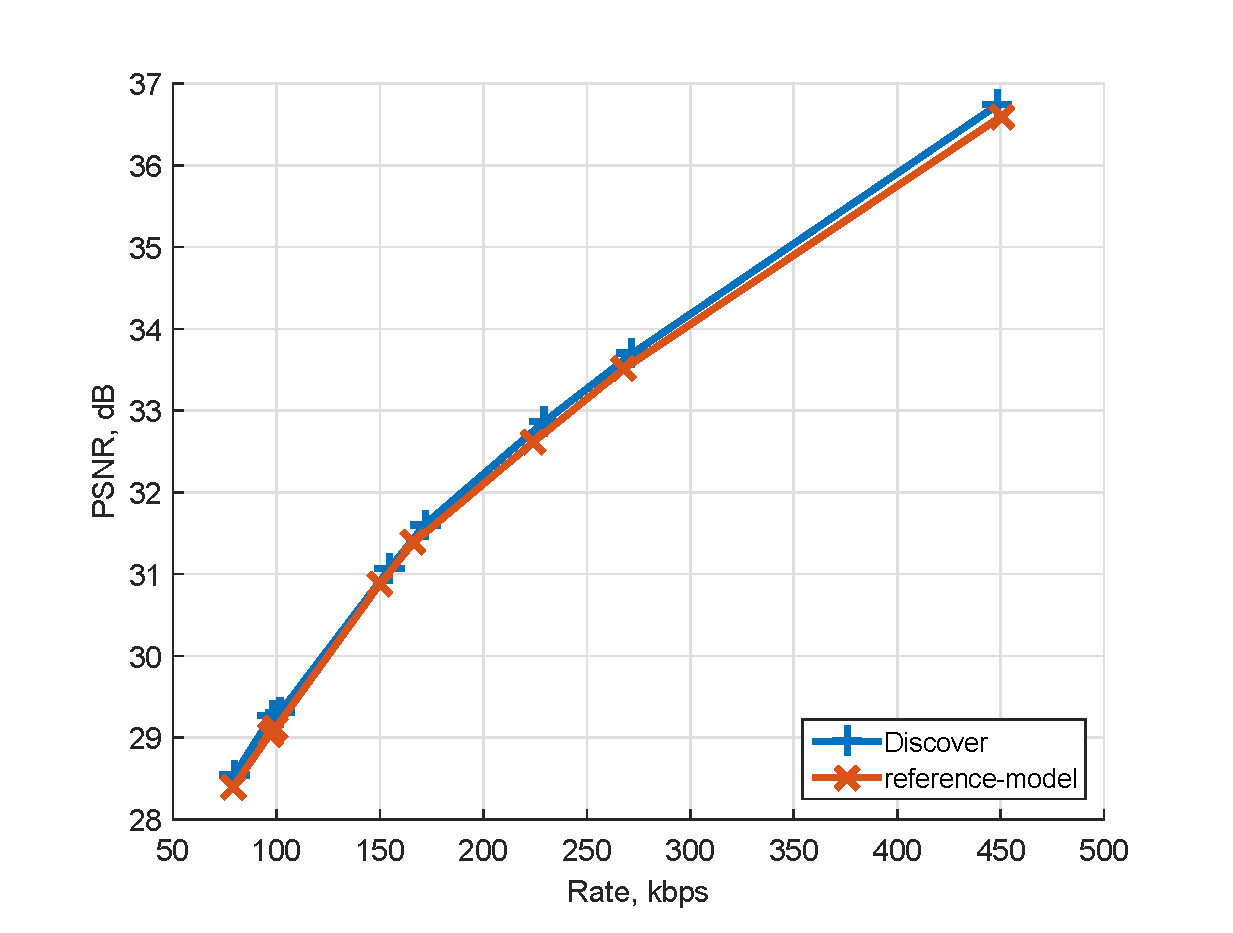
\includegraphics[width=\textwidth]{Chapter4/RefVsDiscover-coastguard-qcif-15Hz} \\ Coastguard
        \end{minipage}
        \begin{minipage}{0.45\textwidth}
            \centering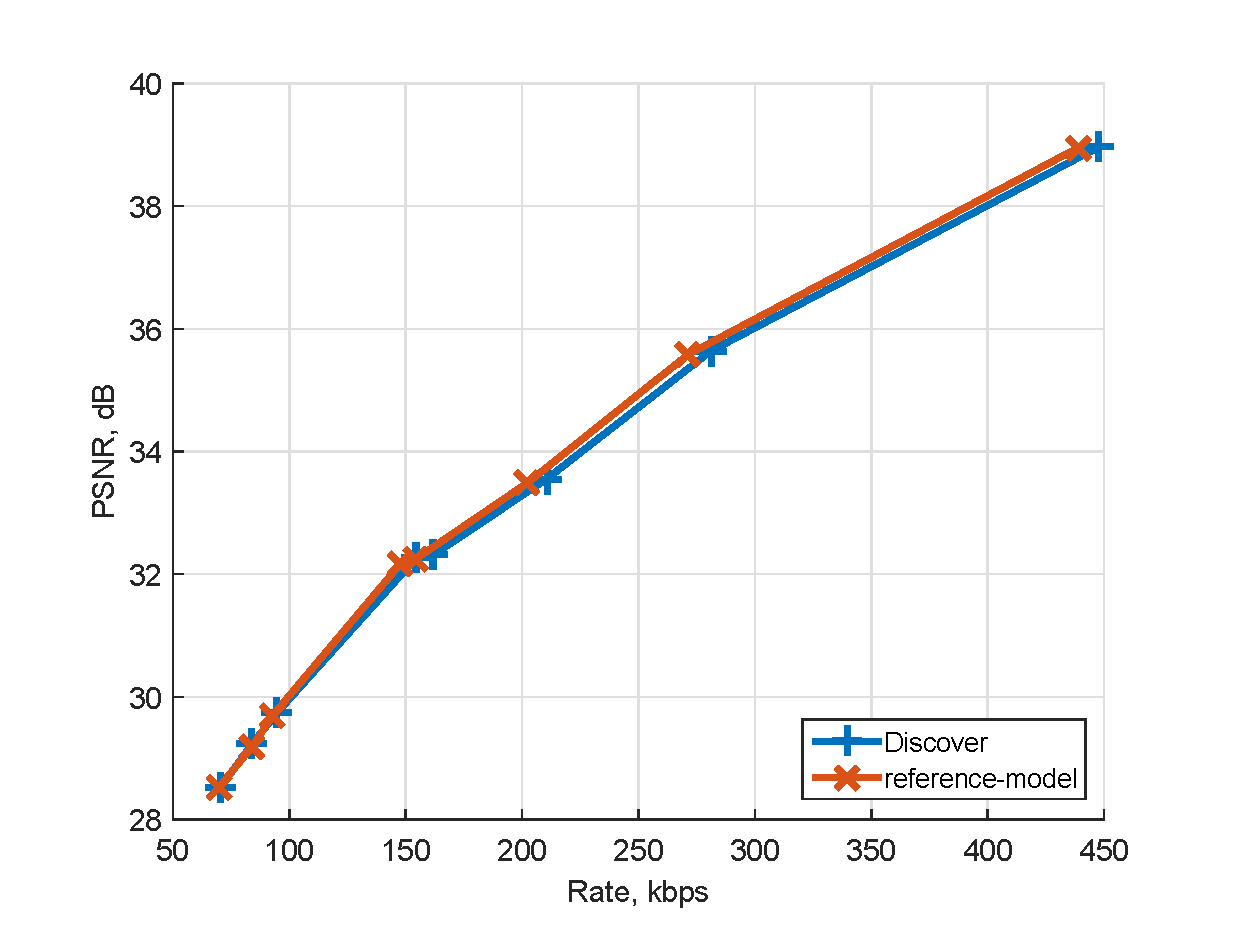
\includegraphics[width=\textwidth]{Chapter4/RefVsDiscover-foreman-qcif-15Hz} \\ Foreman
        \end{minipage}
        \bigskip 
        \begin{minipage}{0.45\textwidth}
            \centering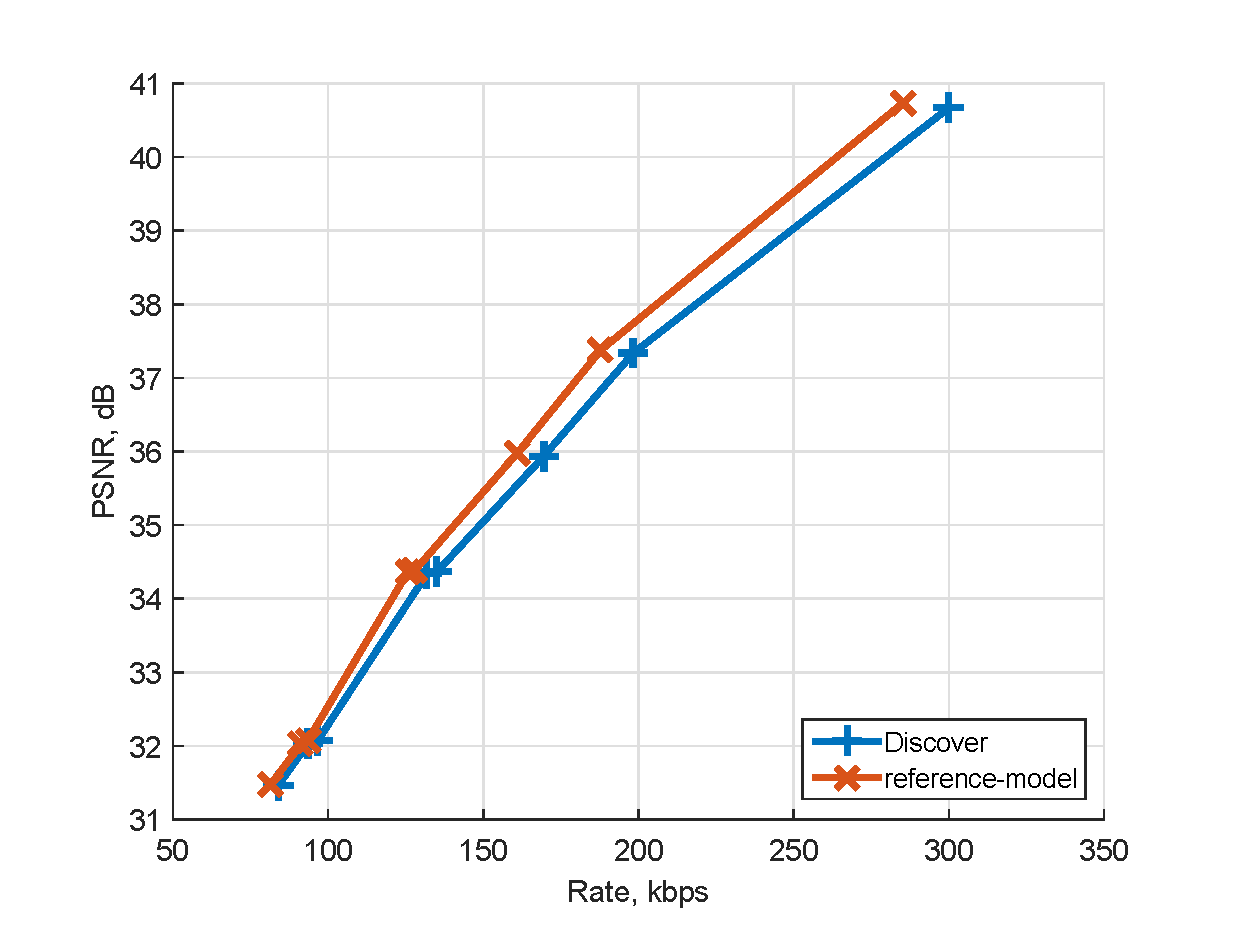
\includegraphics[width=\textwidth]{Chapter4/RefVsDiscover-hall-qcif-15Hz} \\ Hall
        \end{minipage}
        \begin{minipage}{0.45\textwidth}
            \centering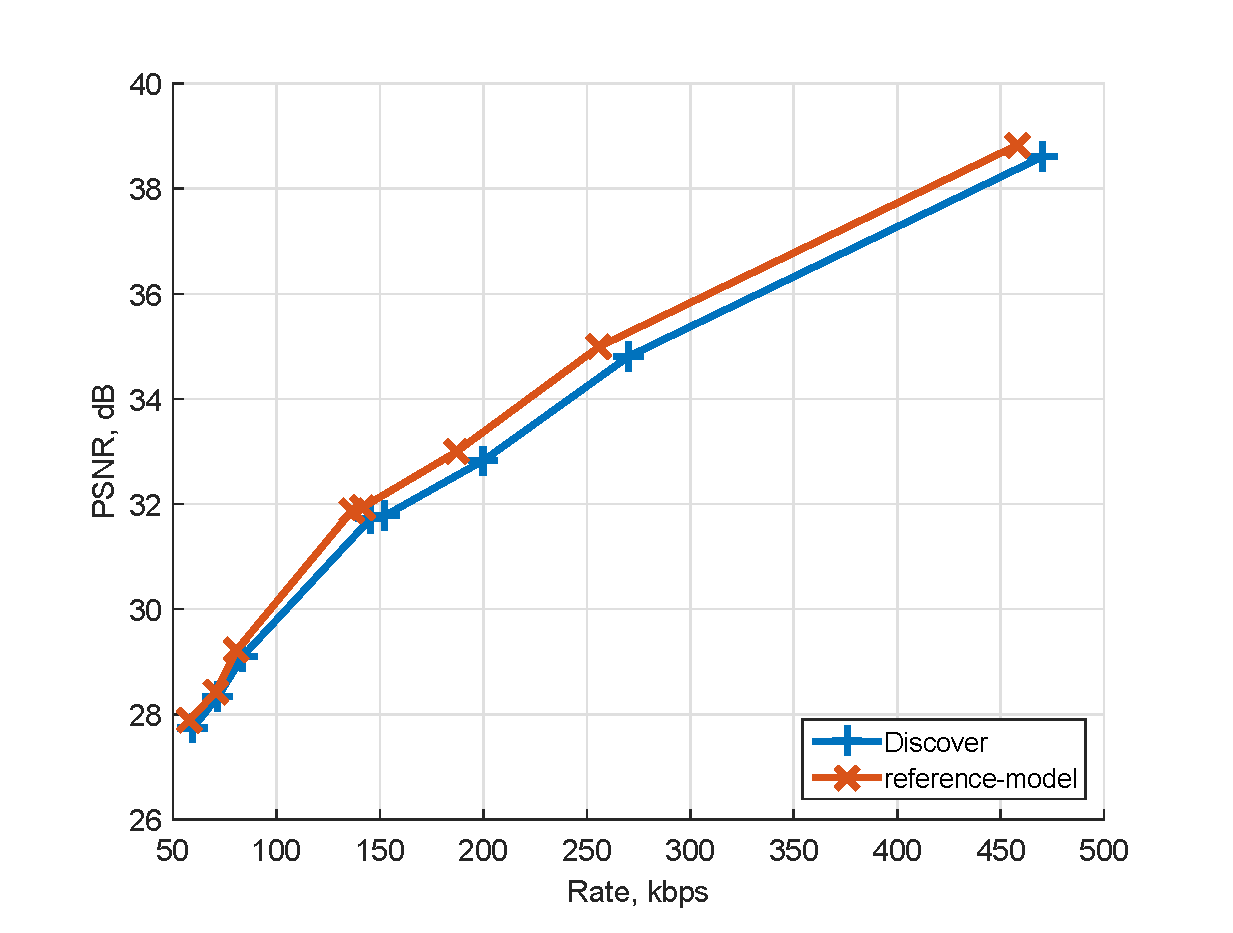
\includegraphics[width=\textwidth]{Chapter4/RefVsDiscover-soccer-qcif-15Hz} \\ Soccer
        \end{minipage}
    \end{center}
    \caption{Сравнение разработанного программного комплекса и кодека DISCOVER по кривым <<скорость-искажение>>}
    \label{fig:CompareReferenceWithDiscover}
\end{figure}

\section{Схема эксперимента для сравнительной оценки разработанных алгоритмов}
\label{chap:ExpResults:SchemeofExperiment}

\subsection{Общие замечания по сравнению алгоритмов обработки видеоинформации в схеме распределенного видеокодирования}
\label{chap:ExpResults:SchemeofExperiment:General}

В настоящее время для проведения сравнительной оценки различных алгоритмов в схеме DVC используется следующий подход~\cite{Huang2008}. Реализуется полная схема распределенного кодека, в рамках которой все алгоритмы во всех модулях считаются зафиксированными. Подобный кодек в дальнейшем считается эталонным. Далее в одном из модулей кодека алгоритм изменяется на тестируемый. Получившийся модифицированный кодек считается тестовым. Эталонный и тестовый кодек прогоняются на одном наборе видеопоследовательностей и получившиеся результаты сравниваются по кривым <<скорость-искажение>>: считается, что чем выше идет кривая, тем лучше работает оцениваемый алгоритм в схеме DVC.

Основная проблема, возникающая при использовании подобного подхода, заключается в том, что модули кодека работают совместно в рамках сложной системы, обладающей высокой эмерджентностью. Например, если оценивать эффективность алгоритма генерации дополнительной информации с использование полной схемы кодирования-декодирования и кривых <<скорость-искажение>>, существенное влияние на итоговый результат оказывают также модуль моделирования виртуального канала, характеристики помехоустойчивого кодирования, метод управления битовой скоростью, процедура восстановления кадров и т.~д. Модуль оценки параметров ошибок межкадрового предсказания в свою очередь принимает на вход аппроксимацию ошибок, рассчитываемую на стороне декодера в модуле генерации дополнительной информации. Наличие подобных зависимостей означает, что сравнительная оценка и демонстрация эффективности разработанных алгоритмов должна выполняться с учетом комплексного влияния всех модулей распределенного видеокодека как друг на друга, так и на итоговый результат. В связи с этим в дальнейших подразделах для каждого разработанного в рамках данной диссертационной работы алгоритма приведено описание и результаты ряда экспериментов, которые необходимо выполнить для того, чтобы продемонстрировать выигрыш от применения данного алгоритма в схеме DVC. В завершение экспериментов приведено сравнение распределенного видеокодека, включающего оба разработанных алгоритма, с кодеком DISCOVER, считающимся базовой реализацией распределенного видеокодека, а также с существующими стандартными алгоритмами сжатия видеоданных.

\subsection{Сравнительная оценка алгоритмов генерации дополнительной информации}
\label{chap:ExpResults:SchemeofExperiment:SIG}

\subsubsection{Методы оценки алгоритмов генерации дополнительной информации}

Как было показано в разделе~\ref{chap:SIG} данной диссертационной работы, в основе алгоритмов генерации дополнительной информации лежит процедура междкадрового предсказания, основанная на временной интерполяции. Чем точнее выполнена интерполяция промежуточных кадров, т.~е. чем больше аппроксимирующий кадр на стороне декодера похож на соответствующий кадр на кодере, тем меньше ошибок межкадрового предсказания будет содержаться в дополнительной информации декодера. Таким образом, для проведения сравнительного анализа алгоритмов генерации дополнительной информации достаточно сравнить результаты временной интерполяции, полученные с использованием базового алгоритма (подраздел~\ref{chap:SIG:ReferenceAlgo}), используемого в программном комплексе, и разработанного алгоритма (подраздел~\ref{chap:SIG:ProposedAlgo}). Следует отметить, что, учитывая приведенные в подразделе~\ref{chap:ExpResults:SchemeofExperiment:General} наблюдения, данное сравнение целесообразно проводить с использованием экспериментов двух типов.
\begin{enumerate}
    \item Сравнение без учета особенностей распределенного кодека. 
    \item Сравнение в рамках распределенного кодека. 
\end{enumerate}
Эксперимент первого типа позволяет судить об алгоритме межкадрового предсказания в целом. Если на данном этапе не наблюдается выигрыша по сравнению с эталонным алгоритмом, то с высокой вероятностью использование данного алгоритма не даст выигрыша и в схеме DVC. Эксперимент второго типа позволяет получить понимание и приблизительные оценки выигрыша/проигрыша от применения тестируемого алгоритма в рамках DVC. Следует отметить, что при разработке эксперимента второго типа особое внимание должно быть уделено вопросам устранения взаимного влияния между модулями распределенного кодека.

\subsubsection{Оценка алгоритма межкадрового предсказания без учета особенностей распределенного кодека}

Для осуществления оценки без учета особенностей распределенного кодека используются существующие методы сравнения алгоритмов временной интерполяции, например в рамках задачи преобразования кадровой скорости, позволяющие оценить визуальное качество интерполяции независимо от того, как данные алгоритмы используются в схеме DVC.

Наиболее распространенным методом оценки алгоритмов временной интерполяции является следующий. Формируется множество тестовых видеопоследовательностей и каждая последовательность прореживается, например, выкидыванием каждого второго кадра. Далее для восстановления выкинутых кадров к каждой паре оставшихся смежных кадров применяется алгоритм временной интерполяции. Затем оригинальные выкинутые кадры сравниваются с интерполированными.

Графики со сравнением покадровых значений критерия PSNR для всех тестовых последовательностей приведены на рисунке~\ref{fig:SIBfPSNR}. Средние значения PSNR, рассчитанные по всем интерполированным кадрам, сведены в таблице~\ref{tab:SIMeanPSNR}.

\begin{table}[H]
    \begin{center}
        \caption{Среднее значение критерия PSNR для промежуточных кадров}
        \label{tab:SIMeanPSNR}
        \begin{tabular}{|c|c|c|}
            \hline
            \textbf{Последовательность} & \textbf{Базовый алгоритм} & \textbf{Предложенный алгоритм} \\
            \hline
            Coastguard 	& $32.13$ 	& $34.66$ \\
            \hline
            Football	& $22.84$	& $23.96$ \\
            \hline
            Foreman 	& $32.55$	& $34.25$ \\
            \hline
            Hall 		& $36.89$ 	& $37.35$ \\
            \hline
            Soccer 		& $25.13$ 	& $27.66$ \\
            \hline
        \end{tabular}
    \end{center}
\end{table}

Из приведенных результатов видно, что разработанный алгоритм, описанный в подразделе~\ref{chap:SIG:ProposedAlgo}, показывает в целом более высокое качество интерполяции, чем базовый алгоритм. Кроме того, следует  отметить тот факт, что величина выигрыша зависит от характеристик видеопоследовательности. Для того, чтобы пояснить данный вывод введем в рассмотрение понятие <<сложности движения>>. Под сложностью движения будем понимать качественную характеристику, зависящую от интенсивности и направления перемещений объектов в видеопоследовательности: чем быстрее и хаотичнее перемещаются объекты, тем более сложное движение. Отсортируем последовательности в соответствии с данным критерием, а также оценим для каждой последовательности выигрыш от применения разработанного алгоритма генерации дополнительной информации с помощью критерия BD-PSNR, позволяющего оценивать разницу между двумя кривыми <<скорость-искажение>>~\cite{Bjontegaard2001}. Результаты данного анализа приведены в таблице~\ref{tab:BDPSNRvsMotionComplexity}.

\begin{table}[H]
    \begin{center}
        \caption{Зависимость выигрыша от сложности движения}
        \label{tab:BDPSNRvsMotionComplexity}
        \begin{tabular}{|c|c|c|}
            \hline
            {\bfseries Последовательность } & {\bfseries Сложность движения} & {\bfseries Разница в значении PSNR, дБ} \\
            \hline
            Coastguard 	& $2$	& $2.53$ \\
            \hline
            Football	& $4$	& $1.12$ \\
            \hline
            Foreman 	& $3$ 	& $1.7$ \\
            \hline
            Hall		& $1$ 	& $0.46$ \\
            \hline
            Soccer 		& $4$ 	& $2.53$ \\
            \hline
        \end{tabular}
    \end{center}
\end{table}

Проанализировав данные в таблице~\ref{tab:BDPSNRvsMotionComplexity}, можно сделать вывод, что чем более сложное движение в видеопоследовательности, тем больше выигрыш от применения разработанного алгоритма генерации дополнительной информации. Полученный результат является ожидаемым, т.~к. на последовательностях с сравнительно простым движением точность временной интерполяции довольно высока у многих алгоритмов, т.~е. число ошибок в дополнительной информации относительно невелико. По мере роста сложности движения, растет и число ошибок. Полученные результаты показывают, что число ошибок в разработанном алгоритме возрастает медленнее, по сравнению с алгоритмом, реализованным в кодеке DISCOVER. Это объясняется тем, что данный алгоритм учитывает модель истинного движения при поиске оптимального векторного поля лучше чем подход, реализованный в DISCOVER.

\begin{figure}[htbp]
    \begin{center}
        \begin{minipage}{0.45\textwidth}
            \centering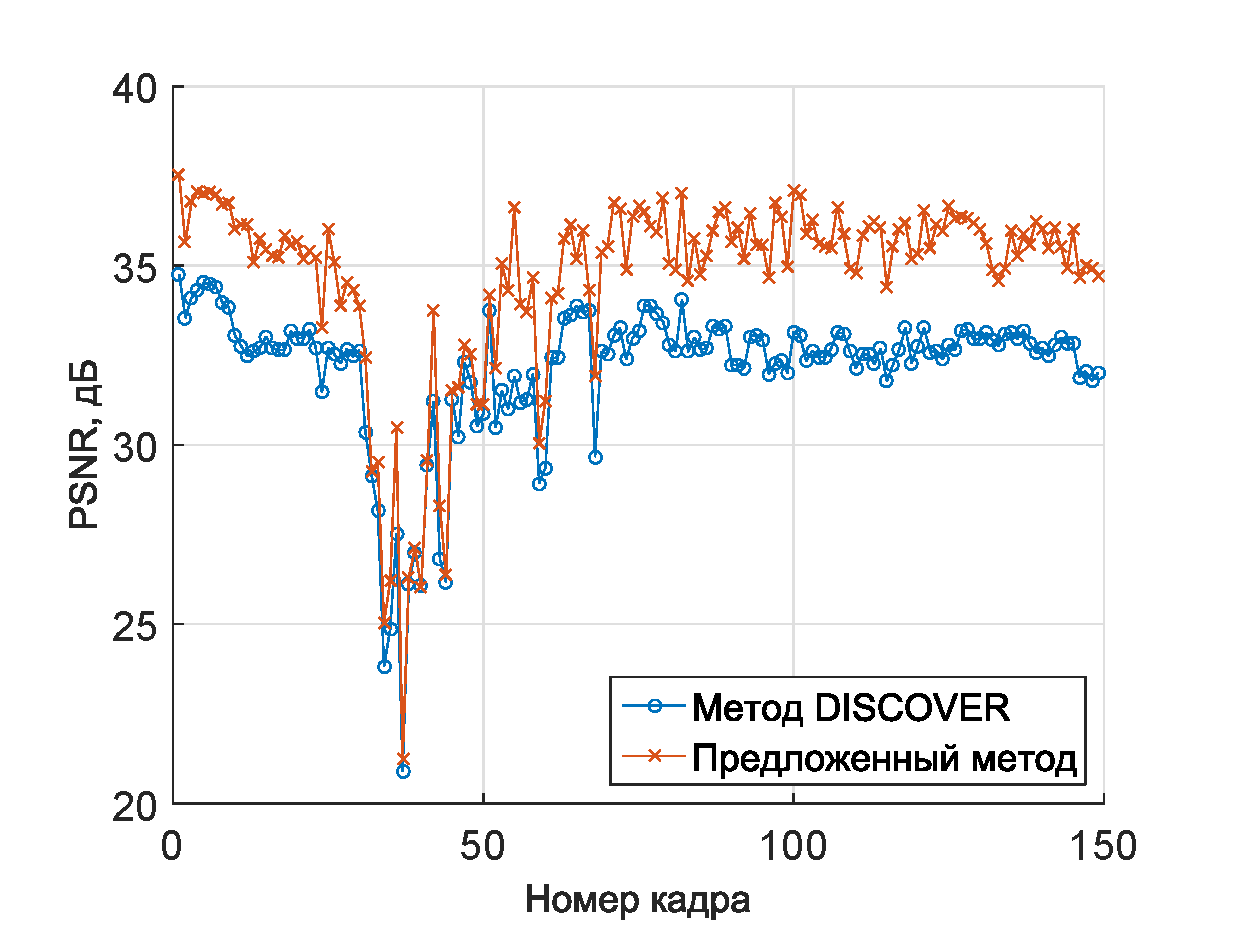
\includegraphics[width=\textwidth]{Chapter4/sigfrc-coastguard-cif-30Hz} \\ Coastguard
        \end{minipage}
        \begin{minipage}{0.45\textwidth}
            \centering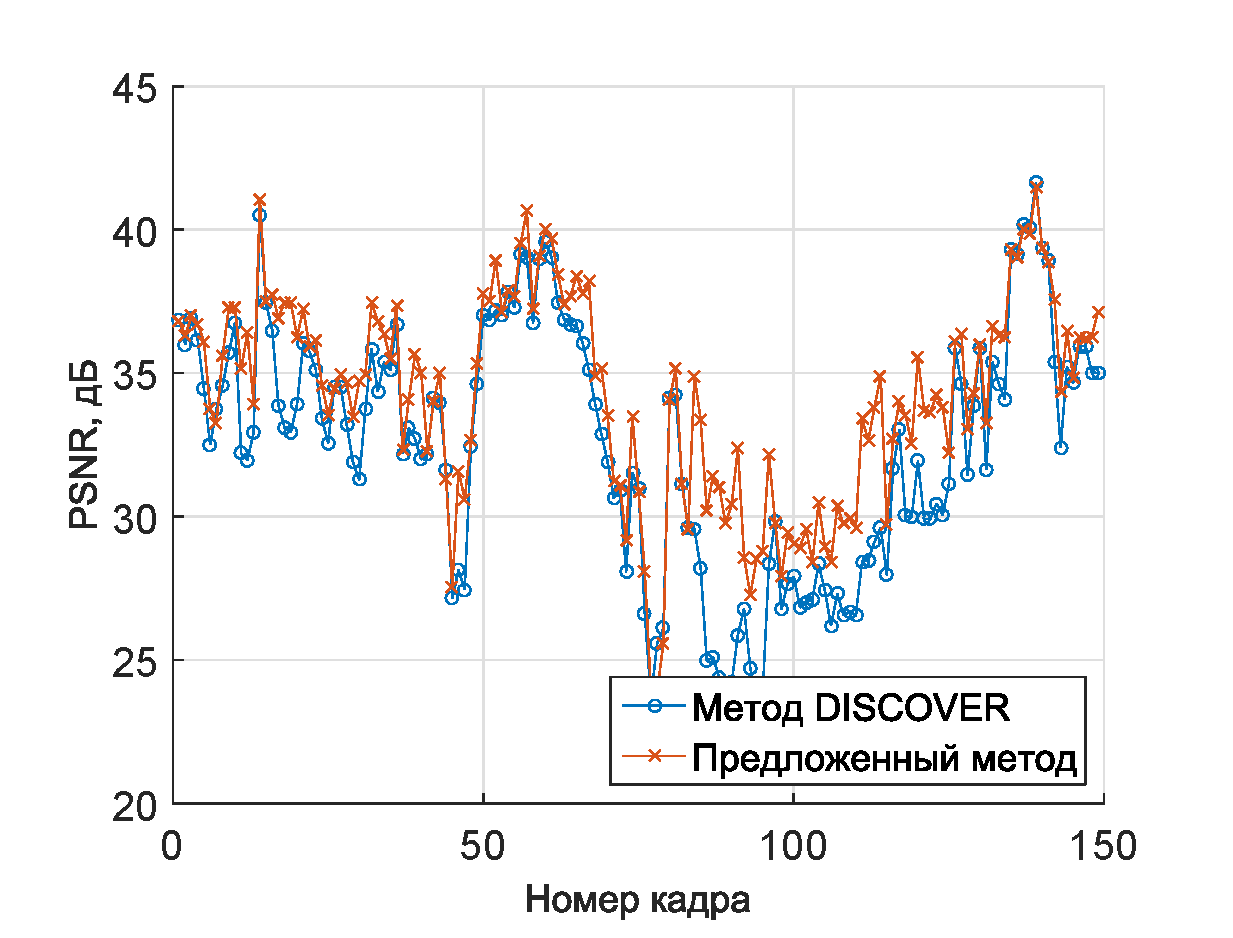
\includegraphics[width=\textwidth]{Chapter4/sigfrc-foreman-cif-30Hz} \\ Foreman
        \end{minipage}
        \\
        \begin{minipage}{0.45\textwidth}
            \centering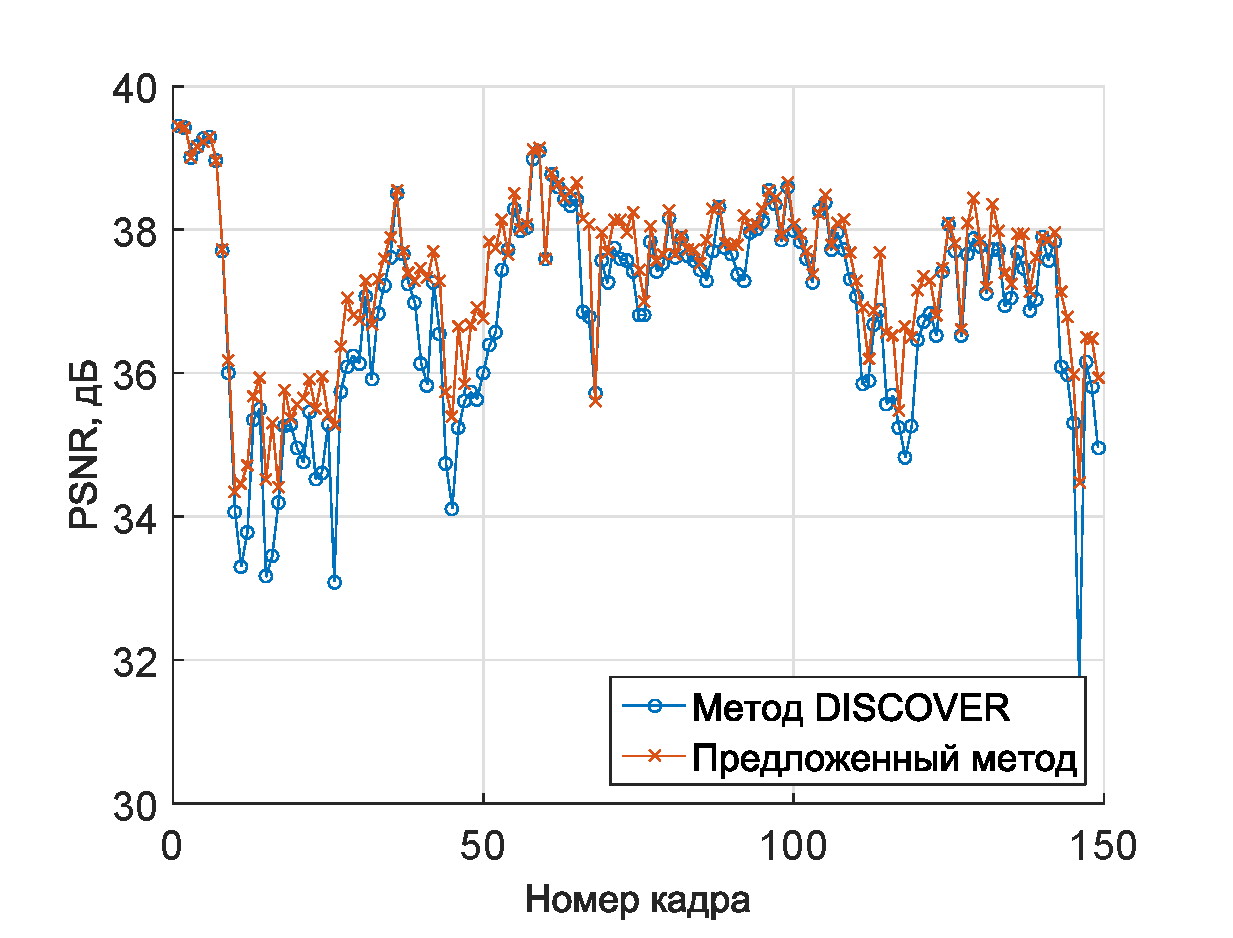
\includegraphics[width=\textwidth]{Chapter4/sigfrc-hall-cif-30Hz} \\ Hall
        \end{minipage}
        \begin{minipage}{0.45\textwidth}
            \centering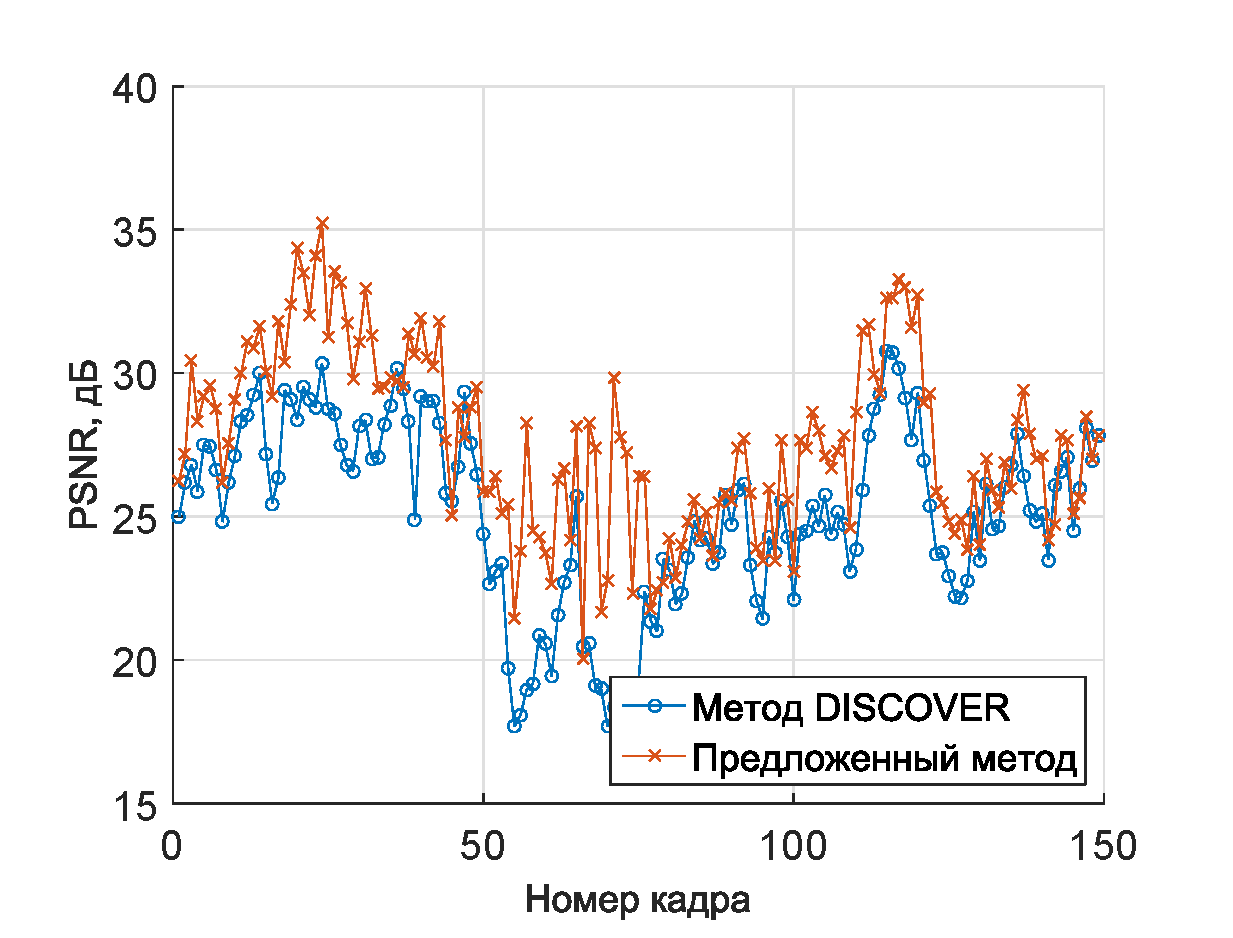
\includegraphics[width=\textwidth]{Chapter4/sigfrc-soccer-cif-30Hz} \\ Soccer
        \end{minipage}
        \\
        \begin{minipage}{0.45\textwidth}
            \centering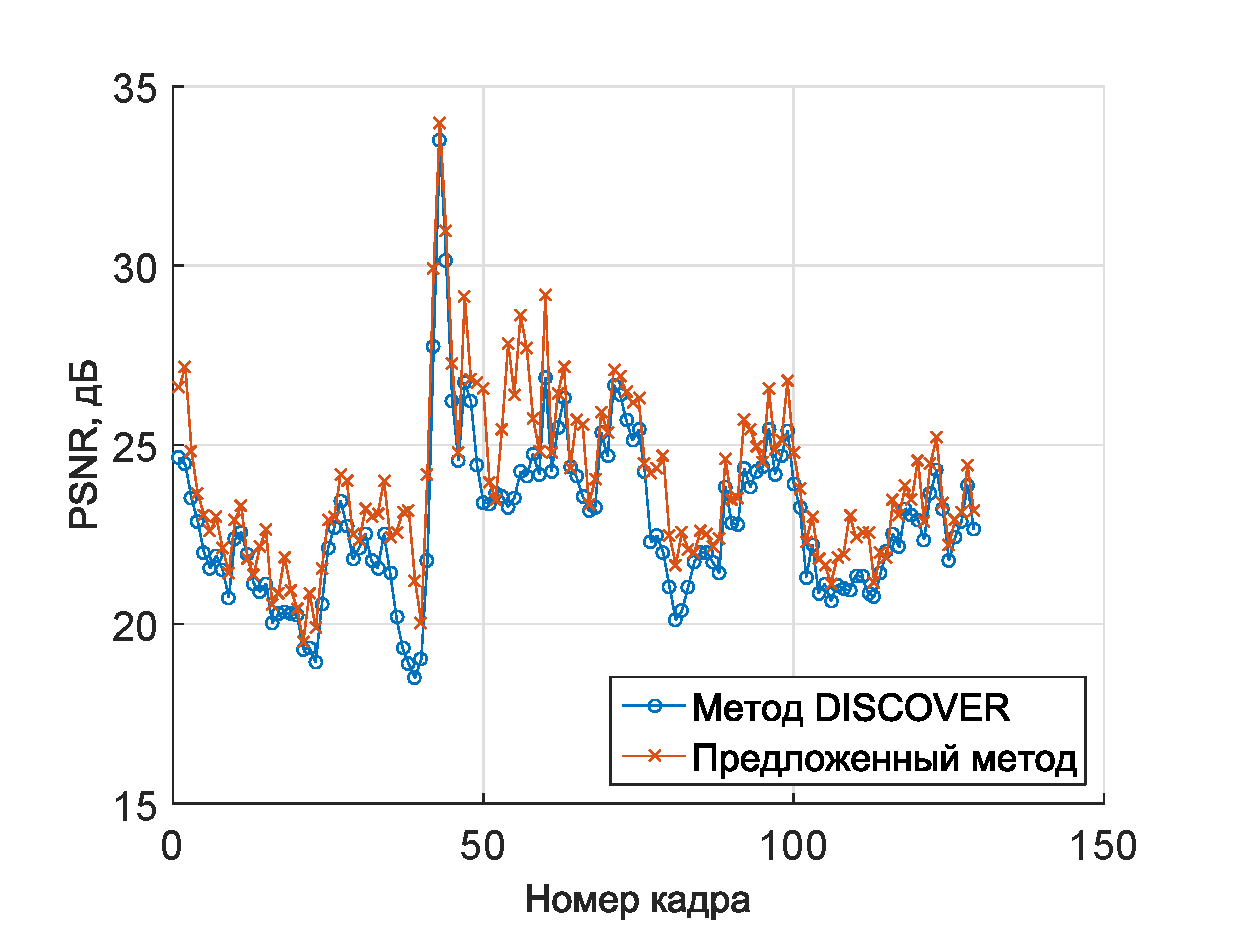
\includegraphics[width=\textwidth]{Chapter4/sigfrc-football-cif-30Hz} \\ Football
        \end{minipage}
    \end{center}
    \caption{Графики PSNR для интерполированных кадров}
    \label{fig:SIBfPSNR}
\end{figure}

\subsubsection{Оценка алгоритма межкадрового предсказания с использованием распределенного кодека}
\label{chap:ExpResults:SchemeofExperiment:SIG:WithDVC}

При оценке алгоритма межкадрового предсказания с использованием распределенного кодека необходимо учесть наблюдения, указанные в подразделе~\ref{chap:ExpResults:SchemeofExperiment:General}, а именно тот факт, что модуль генерации дополнительной информации находится в тесной взаимосвязи с прочими модулями кодека. В настоящей диссертационной работе для решения данной проблемы предлагается использовать следующий подход. Реализуется видеокодек, работающий по схеме, описанной в работах~\cite{Gilmutdinov2012},~\cite{Priborostroenie2013}. Опорные кадры обрабатываются независимо, например в соответствии с алгоритмом, используемым в кодеке DISCOVER. По восстановленным опорным кадрам выполняется межкадровое предсказание промежуточного кадра, результат предсказания выдается в выходной поток в качестве восстановленного промежуточного кадра. Помехоустойчивое кодирование для исправления ошибок в дополнительной информации при этом не выполняется, т.~е. промежуточные кадры обрабатываются только на стороне декодера и дополнительные биты от кодера не требуются. Таким образом, в подобной схеме битовые затраты на передачу промежуточных кадров составляют $0$ бит, а в качестве восстановленных кадров выдаются аппроксимирующие кадры, полученные в процессе генерации дополнительной информации. Схема кодека без обратной связи приведена на рисунке~\ref{fig:ch3:SuaiDvcSIGEstimation}. Суммарные битовые затраты на сжатие всей последовательность определяются только затратами на хранение информации об опорных кадрах. Изменяя степень сжатия опорных кадров, строятся кривые <<скорость-искажение>>, по которым осуществляется сравнительная оценка различных методов алгоритмов временной интерполяции.

\begin{figure}[htb]
\begin{center}
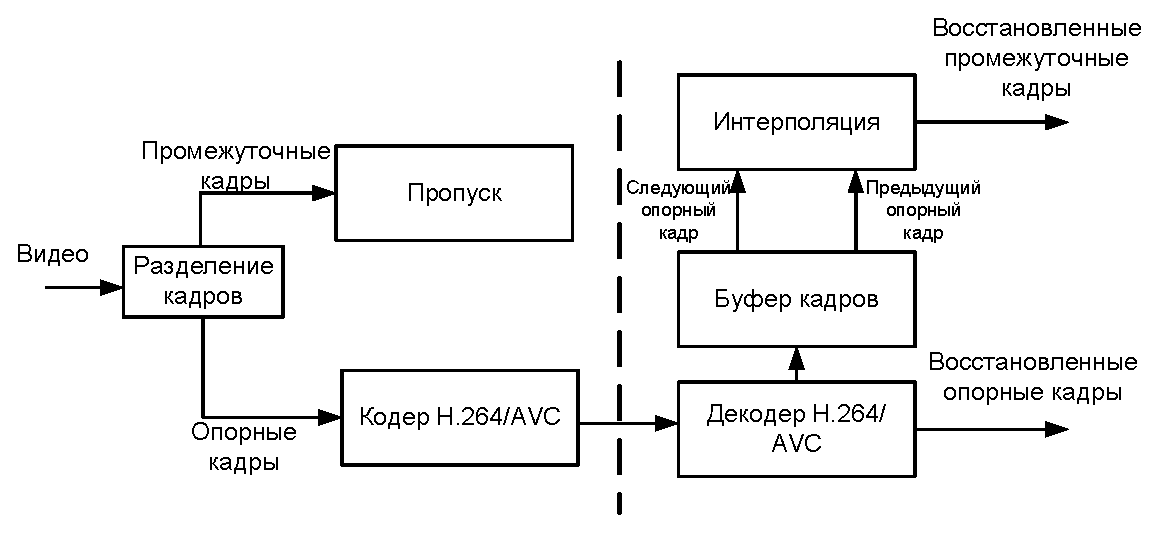
\includegraphics[width=0.9\textwidth]{Chapter4/SuaiDvcSIGEstimation}
\end{center}
\caption{Структурная схема видеокодека для проведения сравнительной оценки алгоритмов генерации дополнительной информации}
\label{fig:ch3:SuaiDvcSIGEstimation}
\end{figure}

Кривые <<скорость-искажение>>, построенные с использованием описанного метода, приведены на рисунке~\ref{fig:ch3:RdSI}. Видно, что разработанный алгоритм межкадрового предсказания выигрывает у базового алгоритма на всех тестовых последовательностях. При этом, как правило, чем более сложное движение в видео, тем более существеннен выигрыш.

\begin{figure}[htbp]
    \begin{center}
        \begin{minipage}{0.45\textwidth}
            \centering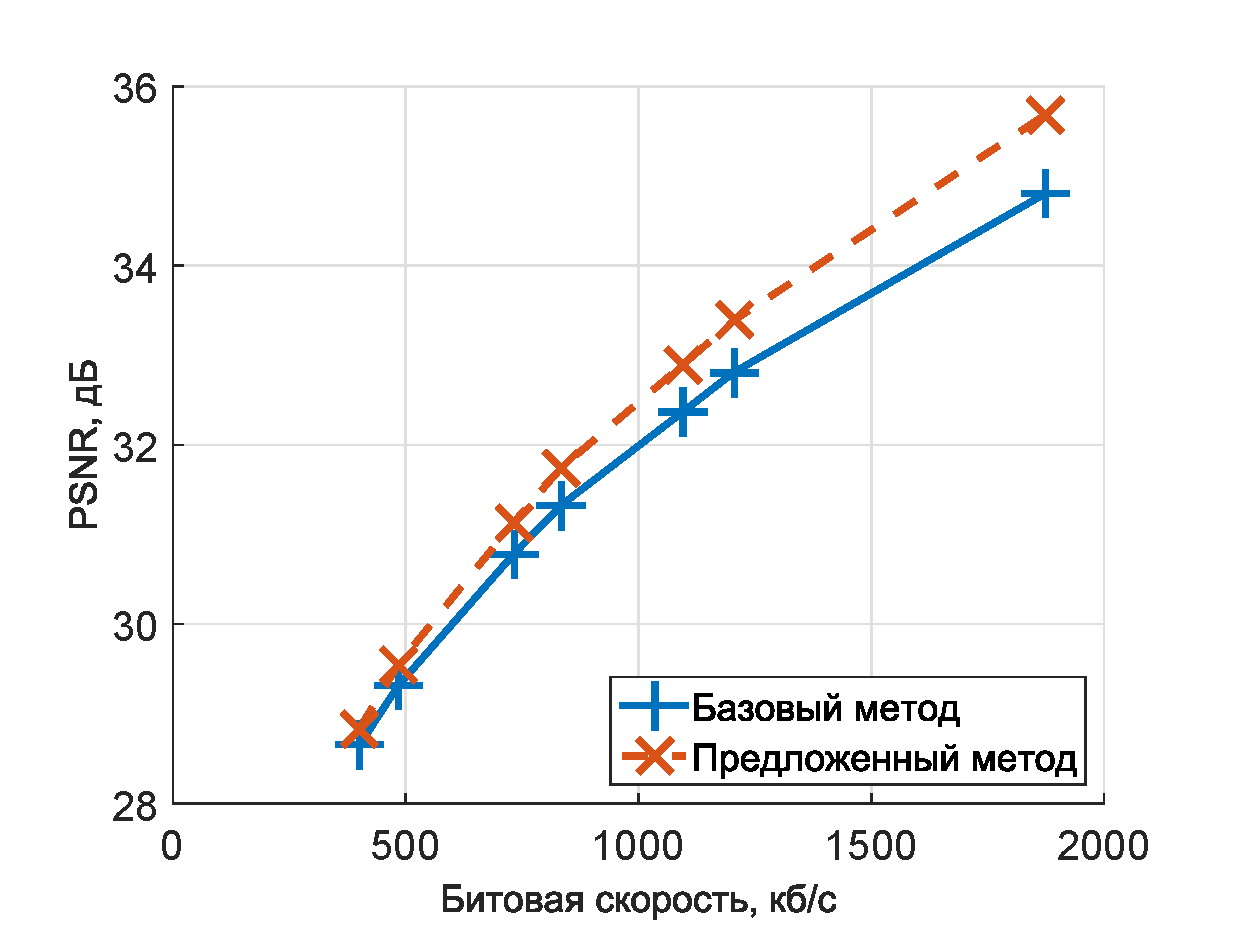
\includegraphics[width=\textwidth]{Chapter4/sigrd-coastguard-cif-30Hz} \\ Coastguard
        \end{minipage}
        \begin{minipage}{0.45\textwidth}
            \centering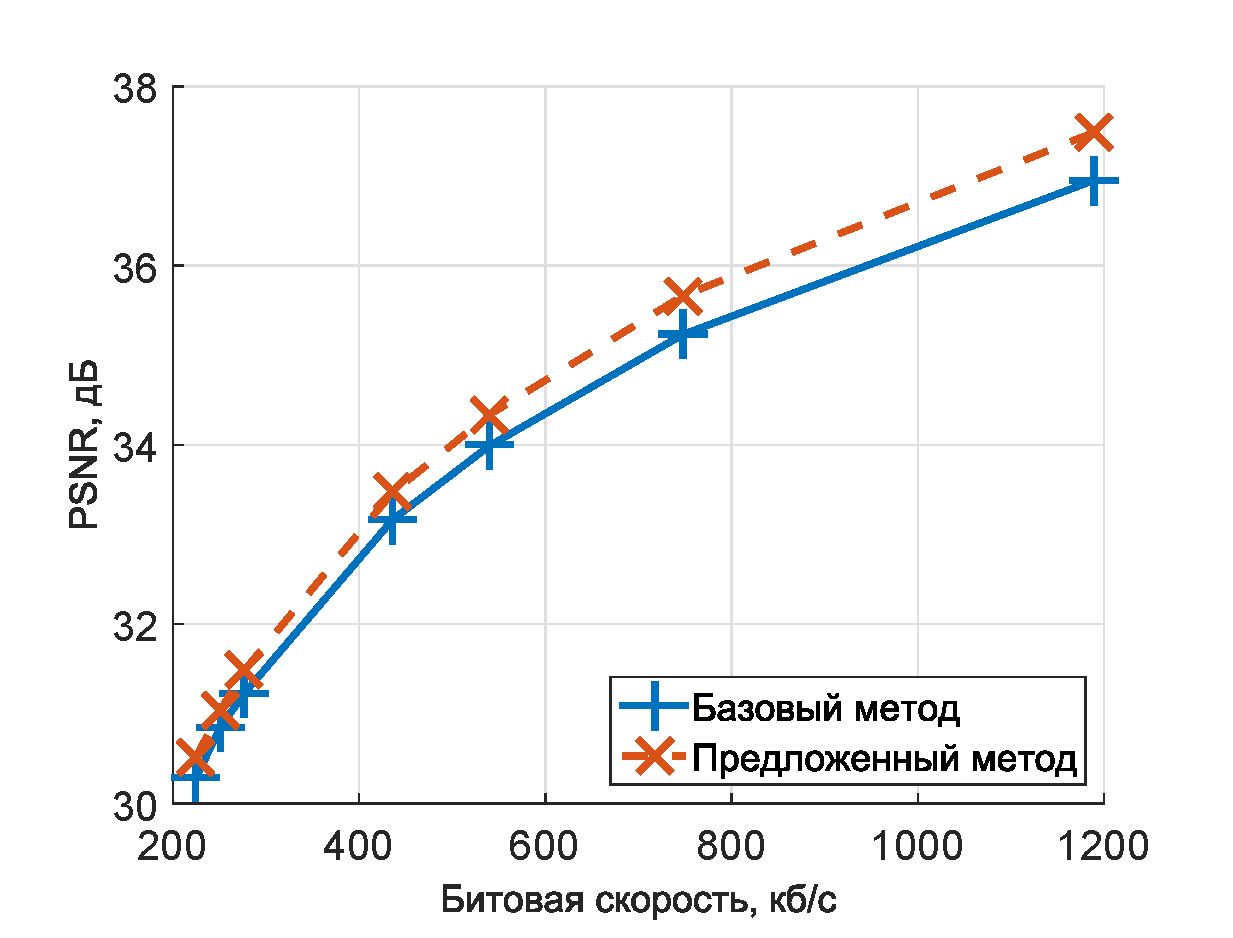
\includegraphics[width=\textwidth]{Chapter4/sigrd-foreman-cif-30Hz} \\ Foreman
        \end{minipage}
        \\
        \begin{minipage}{0.45\textwidth}
            \centering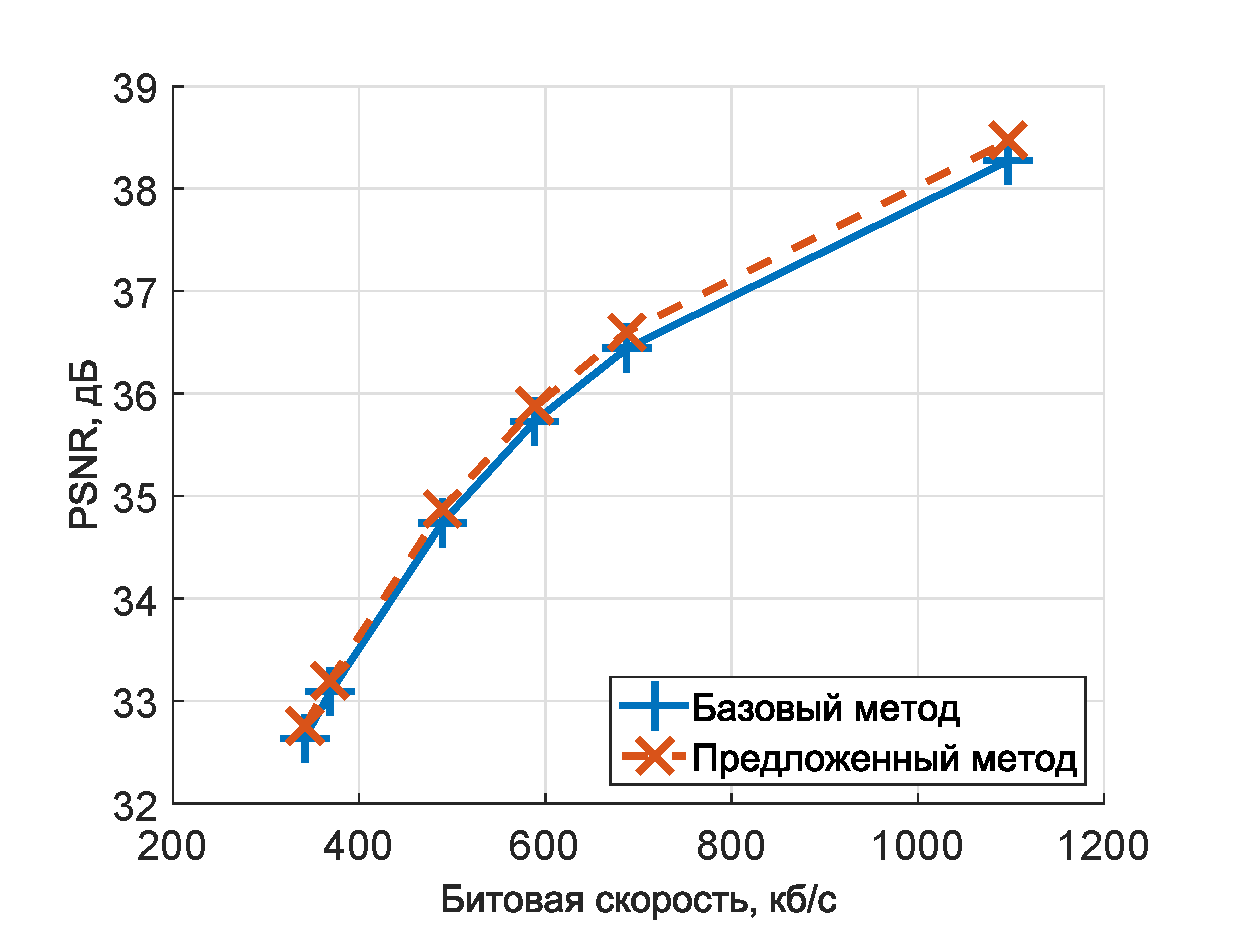
\includegraphics[width=\textwidth]{Chapter4/sigrd-hall-cif-30Hz} \\ Hall
        \end{minipage}
        \begin{minipage}{0.45\textwidth}
            \centering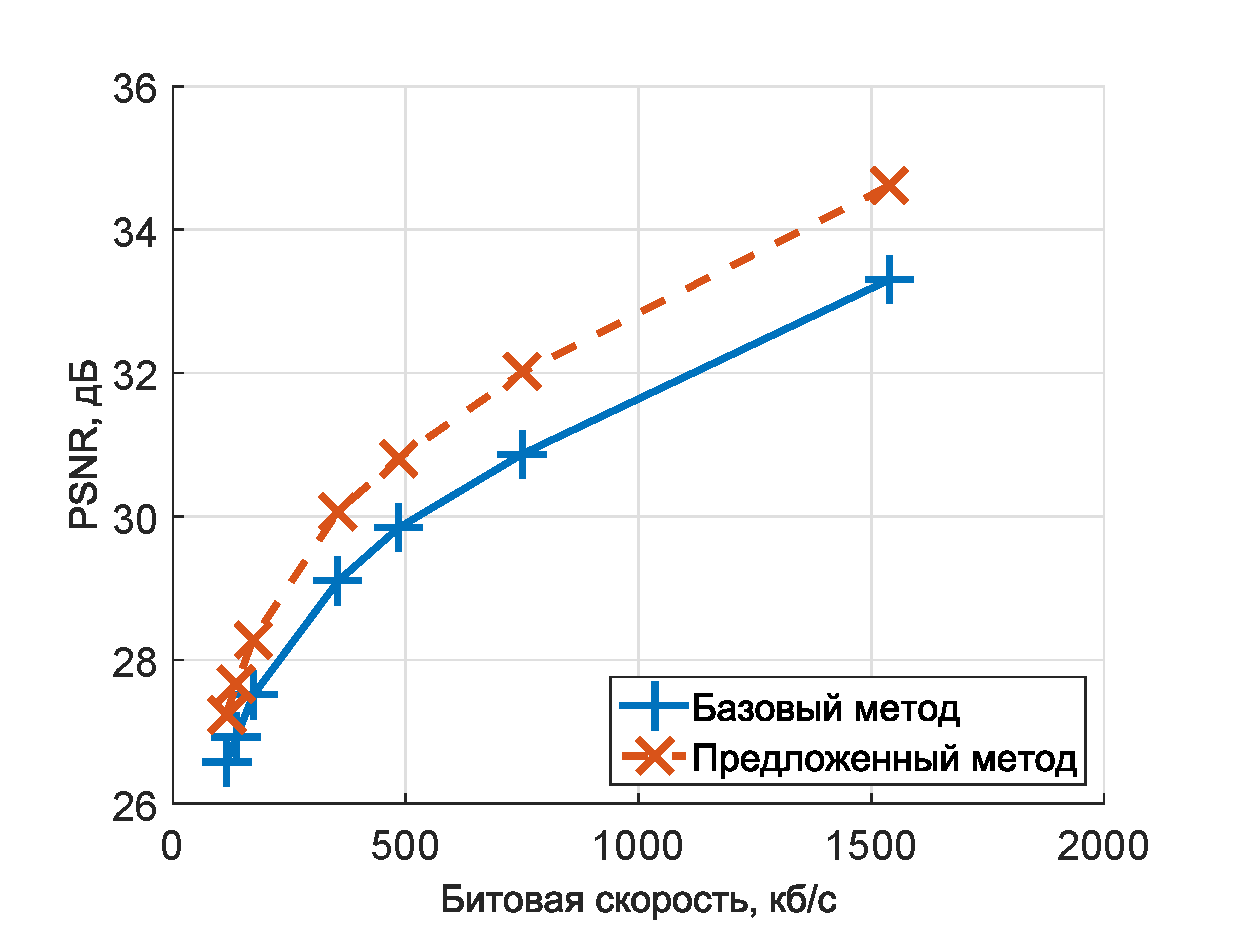
\includegraphics[width=\textwidth]{Chapter4/sigrd-soccer-cif-30Hz} \\ Soccer
        \end{minipage}
        \\
        \begin{minipage}{0.45\textwidth}
            \centering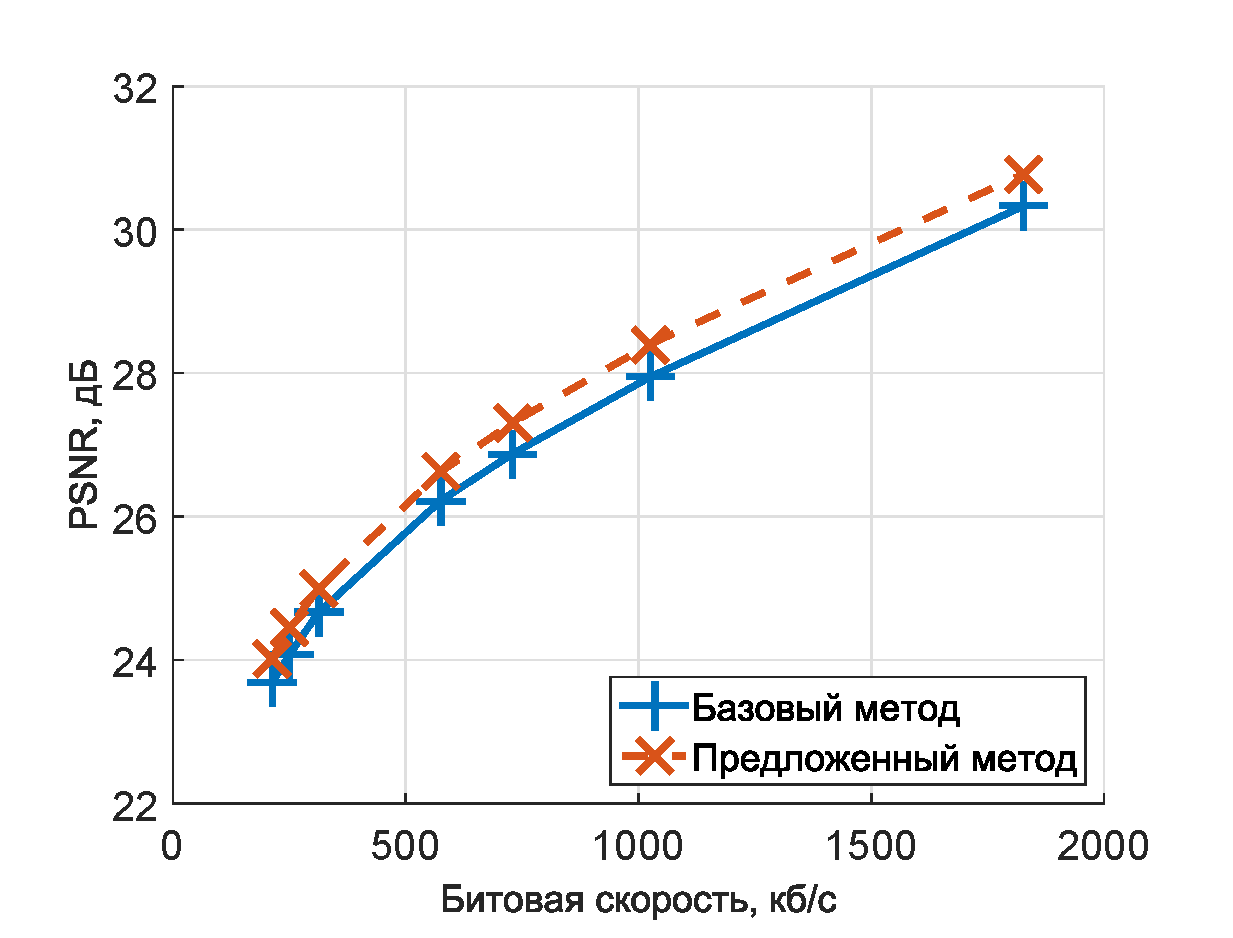
\includegraphics[width=\textwidth]{Chapter4/sigrd-football-cif-30Hz} \\ Football
        \end{minipage}
    \end{center}
    \caption{Результаты сравнения алгоритмов генерации дополнительной информации в рамках распределенного кодека}
    \label{fig:ch3:RdSI}
\end{figure}

Следует отметить, что т.~к. дополнительные биты со стороны кодера для восстановления промежуточных кадров не передаются, кривые <<скорость-искажение>> для упрощенной модели без обратной связи можно построить только для низкого и среднего качества сжатия. Исправление ошибок позволит продлить этот график в область высокого качества за счет повышения битовой скорости.

\subsection{Сравнение алгоритмов оценки параметров ошибок межкадрового предсказания}
\label{chap:ExpResults:SchemeofExperiment:CNM}

При сравнении алгоритмов оценки параметров ошибок межкадрового предсказания необходимо учесть два факта:
\begin{itemize}
    \item способ аппроксимации ошибок межкадрового предсказания на стороне декодера в модуле генерации дополнительной информации;
    \item влияние рассчитанных надежностей символов на последующие процедуры восстановления кадра.
\end{itemize}

Рассмотрим данные факты подробнее. Исследование второго факта, связанного с определением влияния рассчитанных надежностей символов на последующее восстановления кадра, включающее помехоустойчивое декодирование и оптимальное восстановление спектральных коэффициентов, в настоящее время является открытой задачей. На данный момент нет работ, связывающих в какой-либо форме точность оценки параметров ошибок с числом бит, необходимых для их исправления, и, как следствие, качеством восстановленного кадра. Однако, можно сделать разумное предположение, что чем точнее выполнена оценка параметров, тем меньше бит необходимо декодеру для исправления ошибок, и тем выше будет качество восстановленного кадра. Таким образом, будем далее предполагать, что влиянием модуля, выполняющего помехоустойчивое кодирование, при сравнении алгоритмов моделирования виртуального канала можно пренебречь.

Рассмотрим вопросы, связанные с влиянием способа аппроксимации ошибок межкадрового предсказания. В базовой работе~\cite{4498429} по моделированию виртуального канала, а также в ряде других работ, например~\cite{4959735}, в качестве аппроксимации ошибок межкадрового предсказания в спектральной области предлагается  использовать значения преобразованных в спектральную область разностей сопоставления блоков, которые рассчитываются в процедуре оценки движения (подраздел~\ref{chap:CNM:ReferenceAlgo:AlgoDescription}). Следует отметить, что недостатком такого подхода является тот факт, что малое значение ошибки сопоставления блоков не гарантирует отсутствие искажений на аппроксимирующем кадре, и наоборот. Более того, как было показано в подразделе~\ref{chap:SIG:TrueMotionModel}, векторное поле, отражающее истинное движение объектов, является в некотором смысле компромиссом между гладкостью векторов движения и ошибкой сопоставления блоков. Также было отмечено, что малая энергия разностного кадра, которую можно обеспечить с помощью полного перебора в некотором радиусе всех возможных векторов-кандидатов, как правило не соответствует истинному движению. Таким образом, для проведения сравнительного анализа алгоритмов моделирования виртуального канала представляется целесообразным проводить сравнение с использованием экспериментов двух типов.
\begin{enumerate}
    \item Сравнение кривых <<скорость-искажение>>, полученных для настоящих ошибок межкадрового предсказания.
    \item Сравнение кривых <<скорость-искажение>>, полученных для ошибок межкадрового предсказания, оцененных с использованием подхода, описанного в работе~\cite{4498429}.
\end{enumerate}

Эксперимент первого типа позволяет сделать вывод об эффективности алгоритмов моделирования виртуального канала, когда аппроксимация ошибок произведена безошибочно, т.~е. $\hat{\mathbf{n}}^{(b)} \triangleq \mathbf{n}^{(b)}$. Следует отметить, что подобная ситуация является нереализуемой в реальной системе, т.~к. для расчета $\mathbf{n}^{(b)}$ декодер должен заранее обладать информацией о восстановленном промежуточном кадре. Данный сценарий, хоть и нереализуемый на практике, позволяет сравнивать различные алгоритмы моделирования виртуального канала в идеальных условиях, предоставляя информацию о верхней границе для кривых <<скорость-искажение>>, когда все прочие модули в декодере являются зафиксированными.

Эксперимент второго типа позволяет сравнивать эффективность различных алгоритмов моделирования виртуального канала в рамках реальной системы. Отметим, что данное сравнение делается в предположении, что выполнено допущение~\ref{ass:2}, приведенное в подразделе~\ref{chap:CNM:ReferenceAlgo:CommonAssumptions}, т.~е. рассчитанная декодером аппроксимация ошибок в некотором смысле <<похожа>> на реальные ошибки.

Перед тем, как переходить к результатам экспериментов, напомним, что в разработанном алгоритме при решении задачи разделения смеси на втором шаге выполняется поиск параметров законов распределений для заданных скрытых состояний и весов компонент. Будем считать, что функция плотности вероятности ошибок межкадрового предсказания аппроксимируется смесью распределений Лапласа. Данное допущение позволяет использовать при расчете мягкого входа помехоустойчивого декодера и при оптимальном восстановлении кадра те же формулы, что и при использовании базового алгоритма.

Напомним, что модифицированный алгоритм моделирования виртуального канала позволяет учесть свойство пространственной группировки ошибок, характерное в первую очередь для последовательностей со сложным движением. В связи с этим для проведения сравнительного анализа данного алгоритма будем использовать только последовательности Soccer и Football. Кривые <<скорость-искажение>>, построенные для этих последовательностей в рамках экспериментов первого и второго типа приведены на рисунке~\ref{fig:CNM3} и~\ref{fig:CNM4} соответственно. Из приведенных графиков видно, что модифицированный алгоритм выигрывает у базового, однако, следует отметить три факта.

\begin{enumerate}
    \item Основной выигрыш наблюдается в области высокого и среднего качества, на низком качестве кривые <<скорость-искажение>> почти совпадают. Это связано в первую очередь с тем, что на низкой битовой скорости существенное влияние на ошибку межкадрового предсказания вносит шум квантования, причем чем более грубое квантование используется, тем сильнее этот вклад. Данное влияние никак не учитывается в базовом и модифицированном алгоритме.
    \item Значение выигрыша, полученное для экспериментов первого типа, существенно превышает значение выигрыша, полученное для экспериментов второго типа. Это означает, что на практике допущение о похожести аппроксимации ошибок на реальные значения ошибок выполняется не в полной мере.
    \item Выигрыш от применения модифицированного алгоритма в целом незначителен. Данный факт связан с тем, что не совсем корректно аппроксимировать ошибки межкадрового предсказания в областях с низким качеством интерполяции распределением Лапласа с нулевым математическим ожиданием. Расширение алгоритма на другие распределения является предметом дальнейших исследований. В целом можно сделать вывод, что результаты, полученные для модифицированного алгоритма, подтверждают обоснованность концепции моделирования виртуального канала с использованием независимых регионов.
\end{enumerate}

\begin{figure}[htbp]
    \begin{center}
        \begin{minipage}{0.45\textwidth}
            \centering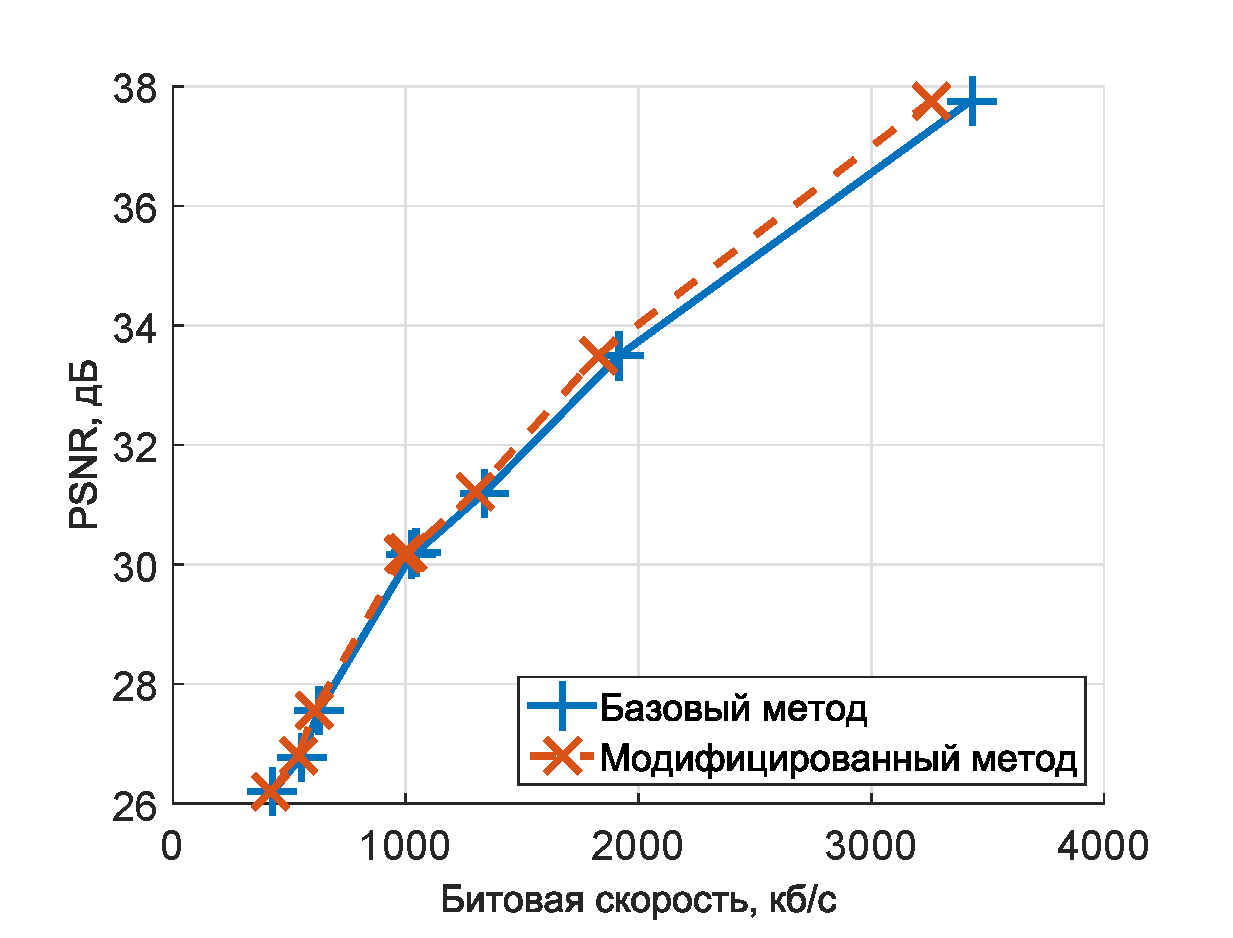
\includegraphics[width=\textwidth]{Chapter4/cnmrdoracle-football-cif-30Hz} \\ Football
        \end{minipage}
        \begin{minipage}{0.45\textwidth}
            \centering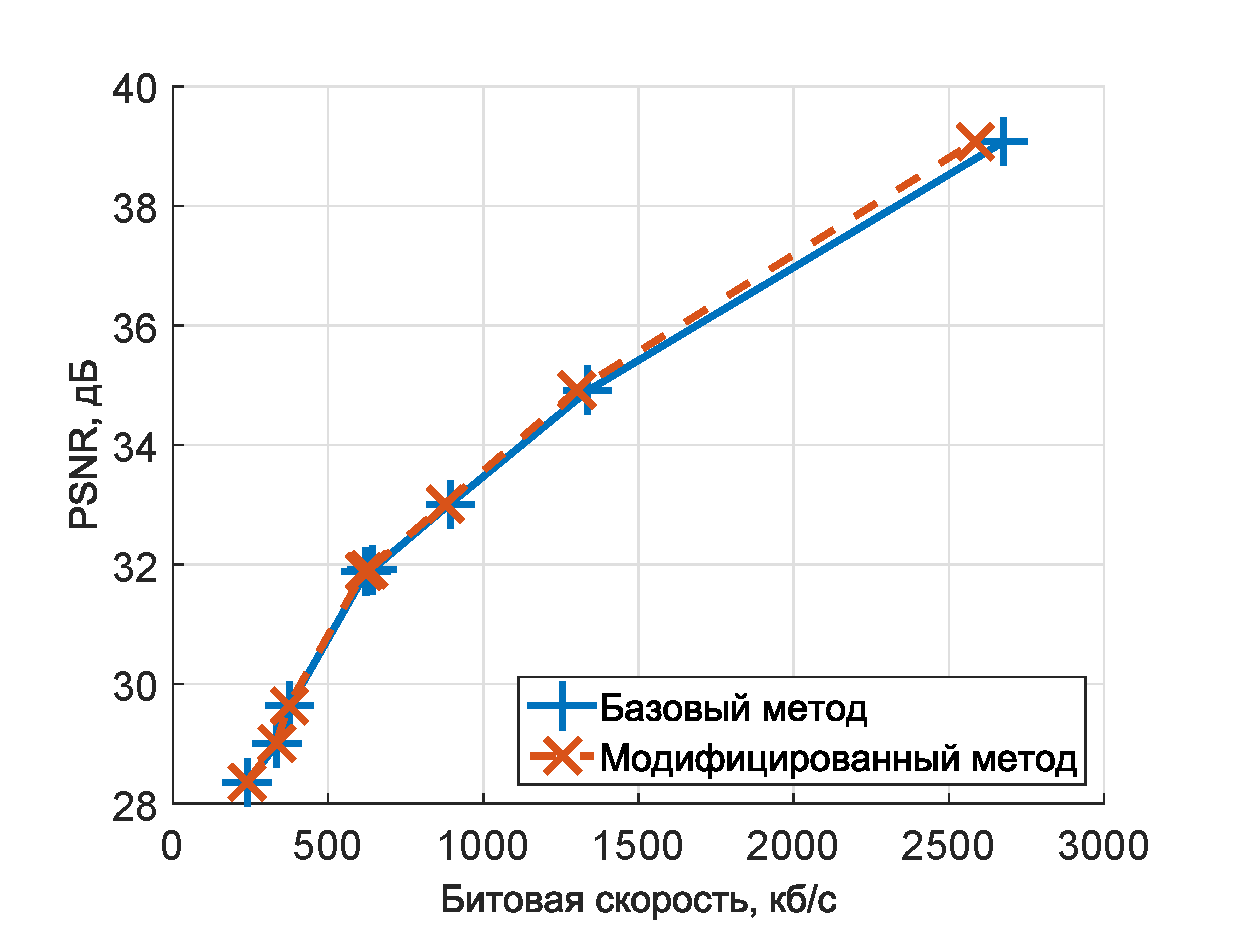
\includegraphics[width=\textwidth]{Chapter4/cnmrdoracle-soccer-cif-30Hz} \\ Soccer
        \end{minipage}
    \end{center}
    \caption{Кривые <<скорость-искажение>>, полученные для сравнения алгоритмов моделирования виртуального канала в рамках экспериментов первого типа}
    \label{fig:CNM3}
\end{figure}

\begin{figure}[htbp]
    \begin{center}
        \begin{minipage}{0.45\textwidth}
            \centering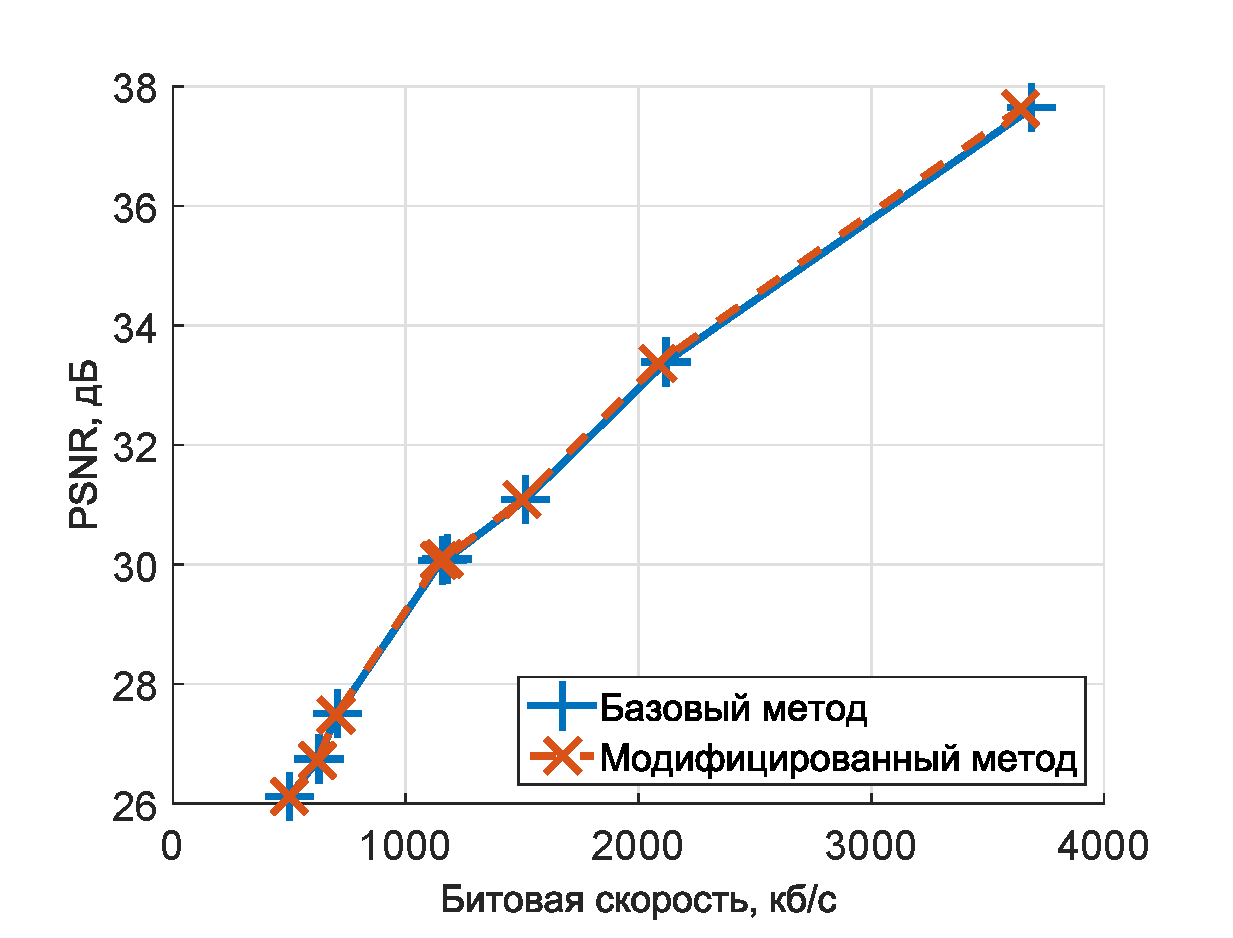
\includegraphics[width=\textwidth]{Chapter4/cnmrd-football-cif-30Hz} \\ Football
        \end{minipage}
        \begin{minipage}{0.45\textwidth}
            \centering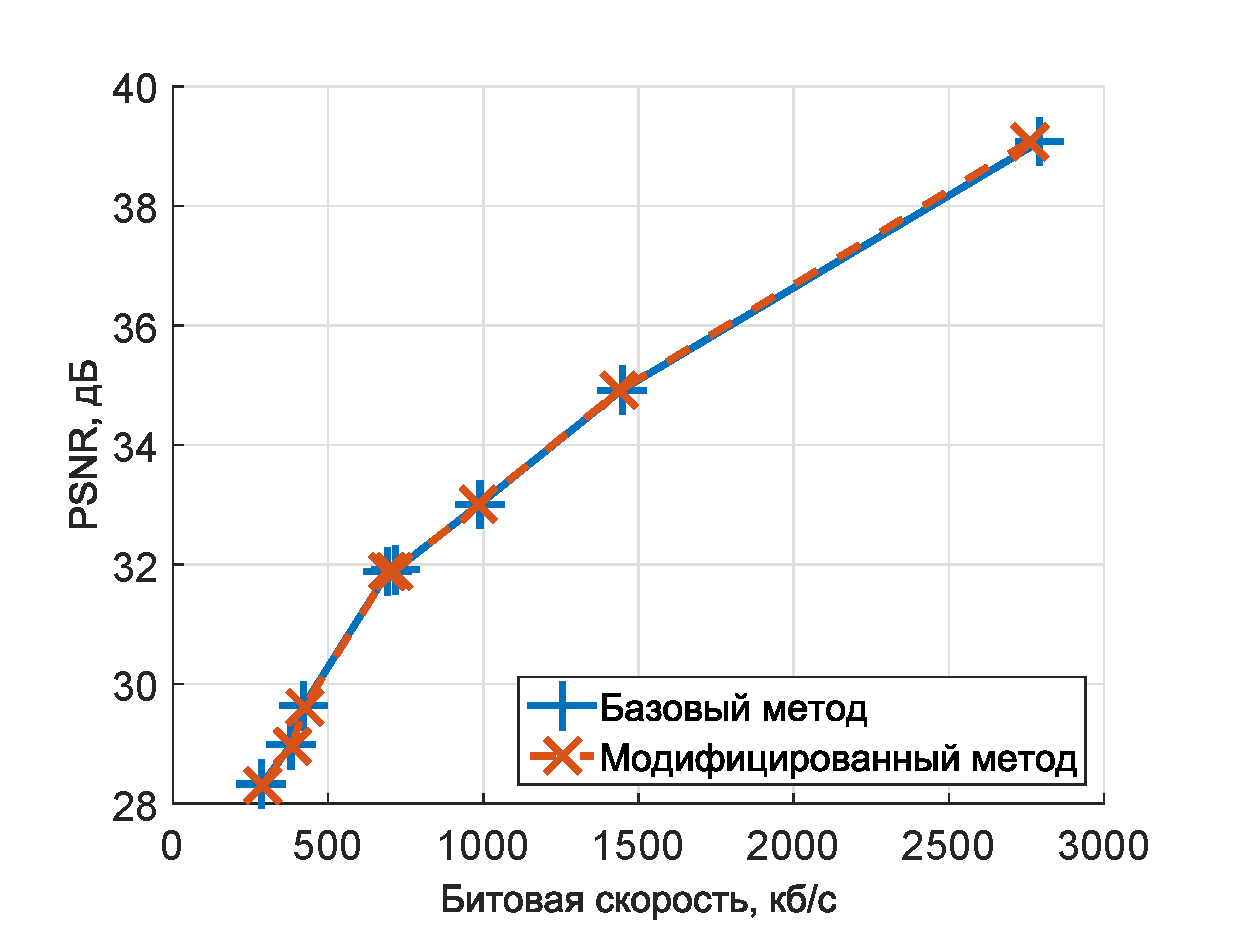
\includegraphics[width=\textwidth]{Chapter4/cnmrd-soccer-cif-30Hz} \\ Soccer
        \end{minipage}
    \end{center}
    \caption{Кривые <<скорость-искажение>>, полученные для сравнения алгоритмов моделирования виртуального канала в рамках экспериментов второго типа}
    \label{fig:CNM4}
\end{figure}

\begin{table}[htbp]
    \begin{center}
        \caption{Значение критерия BD-RATE для экспериментов первого типа}
        \label{tab:CNMComparisonOracleBDRate}
        \begin{tabular}{|c|c|}
            \hline
            {\bfseries Последовательность } & {\bfseries BD-Rate, \%} \\
            \hline
            Football	& $3.8$	\\
            \hline
            Soccer 		& $2.2$	\\
            \hline
        \end{tabular}
    \end{center}
\end{table}

\begin{table}[htbp]
    \begin{center}
        \caption{Значение критерия BD-RATE для экспериментов первого типа}
        \label{tab:CNMComparisonBDRate}
        \begin{tabular}{|c|c|}
            \hline
            {\bfseries Последовательность } & {\bfseries BD-Rate, \%} \\
            \hline
            Football	& $1$	\\
            \hline
            Soccer 		& $0.6$	\\
            \hline
        \end{tabular}
    \end{center}
\end{table}

\section{Сравнительный анализ разработанного алгоритма распределенного видеокодирования}

В данном подразделе приведены результаты сравнения разработанной программной модели распределенного видеокодека с существующими алгоритмами сжатия: 
\begin{itemize}
    \item кодек стандарта H.264, работающий в режиме Intra;
    \item кодек стандарта H.264, работающий в режиме Inter;
    \item кодек стандарта H.264, работающий в режиме Inter No Motion;
    \item кодек DISCOVER.
\end{itemize}

Во всех тестах в качестве кодека использовалась эталонная реализация JM версии 9.5. В режиме H.264 Intra все кадры обрабатывались как ключевые. В остальных режимах использовался режим IBIB, т.е. каждый второй кадр обрабатывался как ключевой. Отметим, что в режиме H.264 Inter межкадровое предсказание и устранение временной избыточности осуществляется кодером, т.~е. данную кривую можно рассматривать в качестве примера для совместного кодирования-декодирования зависимых источников.

Результаты сравнения по кривым <<скорость-искажение>> приведены на рисунке~\ref{fig:FinalDvcComparisonResults}. На всех последовательностях из тестового множества разработанная программная модель выигрывает у кодека DISCOVER в среднем. При этом оба кодека проигрывают на всех последовательностях кодеку H.264 Inter. На последовательностях с высокой сложностью движения (Football и Soccer) и Discover, и разработанный алгоритм проигрывают как H.264 Inter, так и H.264 Intra. Однако следует отметить, что на высоком качестве для последовательности Soccer разработанный алгоритм, в отличие от DISCOVER, показывает качество, близкое к H.264 Intra.
Результаты сравнения разработанного программного комплекса и кодека DISCOVER по критерию BD-RATE приведены в таблице~\ref{tab:ComparisonWithDiscover}. Можно сделать вывод, что применение разработанных алгоритмов позволяет снизить битовые затраты на $4-16 \%$, причем чем сложнее движение в видеопоследовательности, тем больше выигрыш.

\begin{figure}[htbp]
    \begin{center}
        \begin{minipage}{0.45\textwidth}
            \centering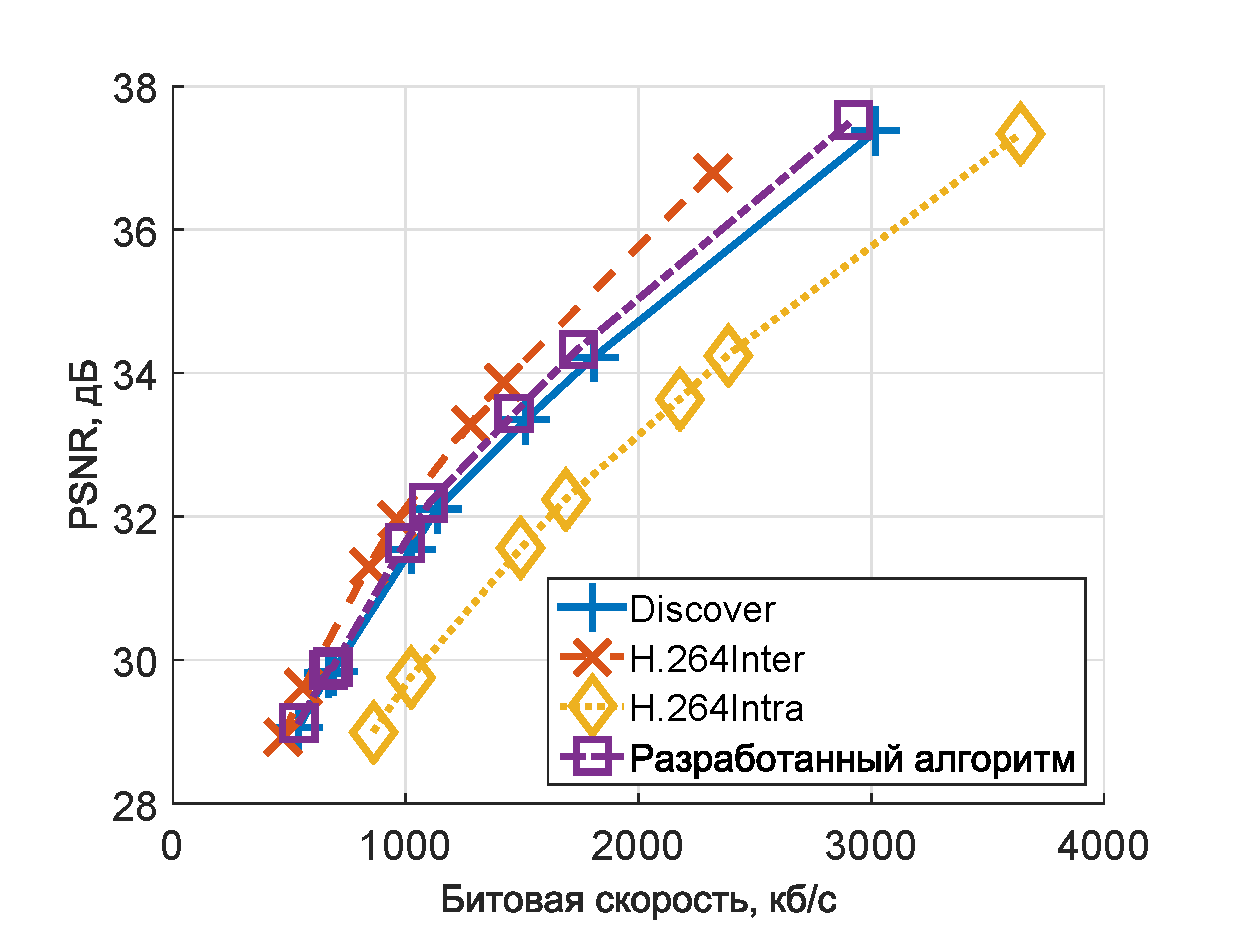
\includegraphics[width=\textwidth]{Chapter4/rdfinal-coastguard-cif-30Hz} \\ Coastguard
        \end{minipage}
        \begin{minipage}{0.45\textwidth}
            \centering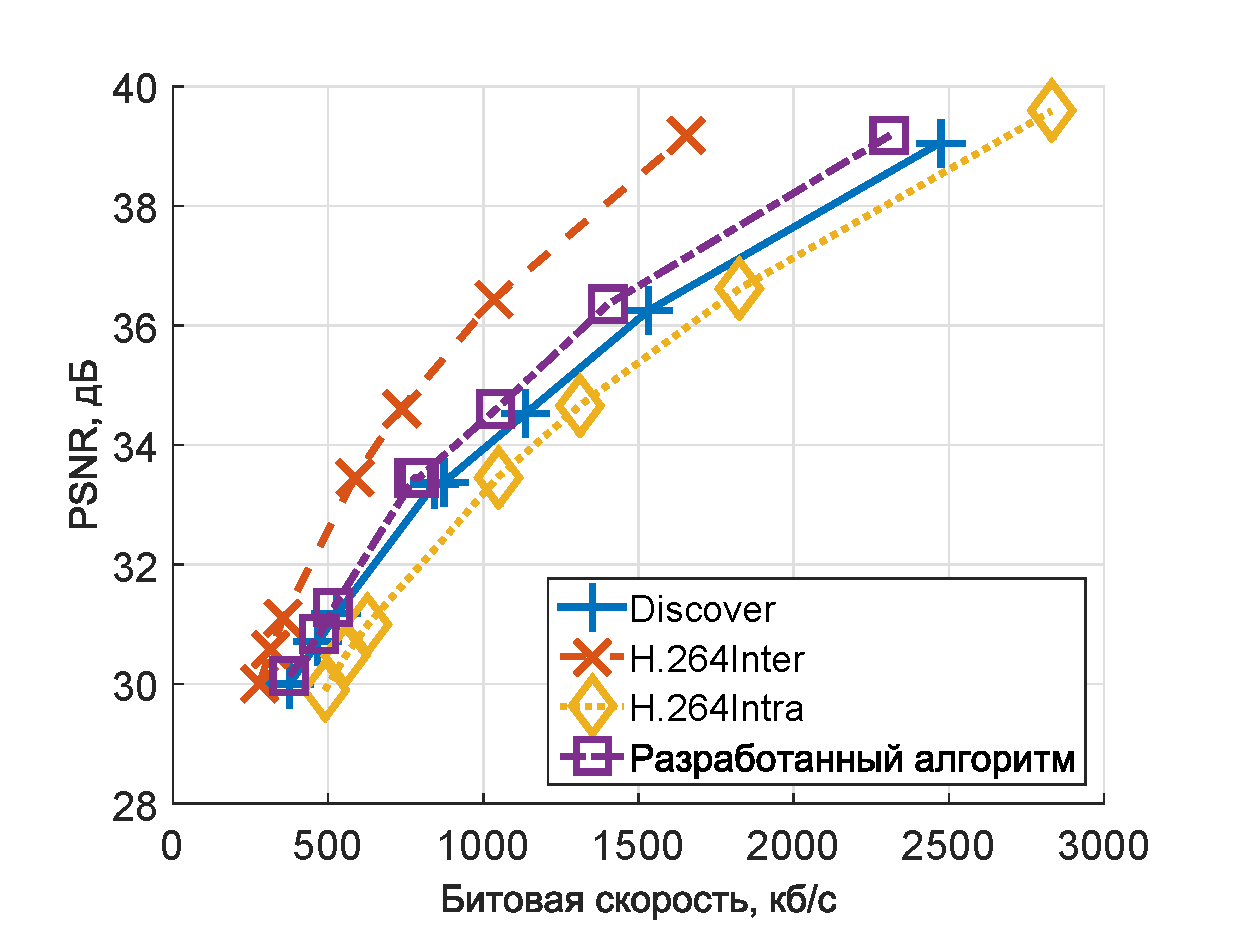
\includegraphics[width=\textwidth]{Chapter4/rdfinal-foreman-cif-30Hz} \\ Foreman
        \end{minipage}
        \\
        \begin{minipage}{0.45\textwidth}
            \centering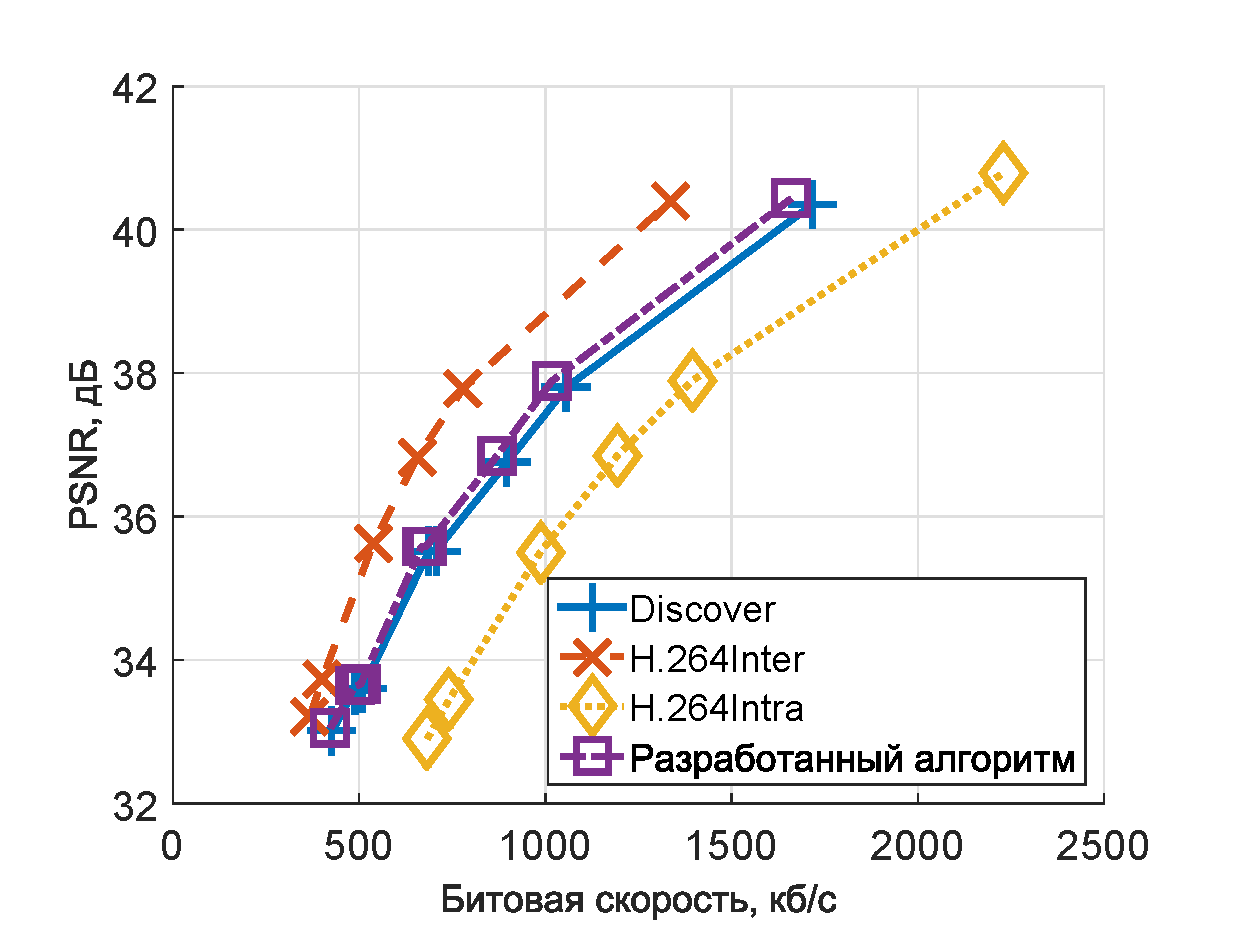
\includegraphics[width=\textwidth]{Chapter4/rdfinal-hall-cif-30Hz} \\ Hall
        \end{minipage}
        \begin{minipage}{0.45\textwidth}
            \centering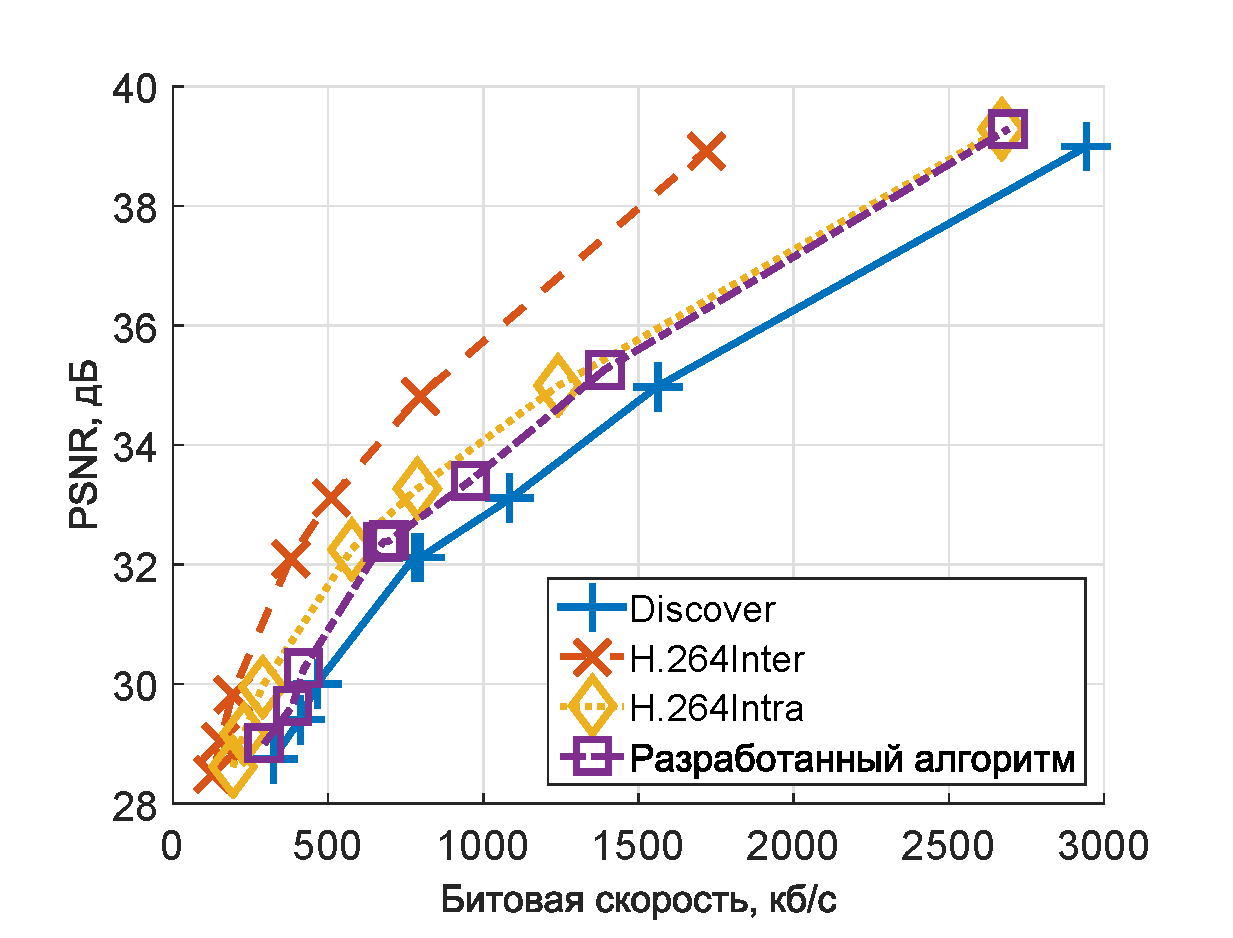
\includegraphics[width=\textwidth]{Chapter4/rdfinal-soccer-cif-30Hz} \\ Soccer
        \end{minipage}
        \\
        \begin{minipage}{0.45\textwidth}
            \centering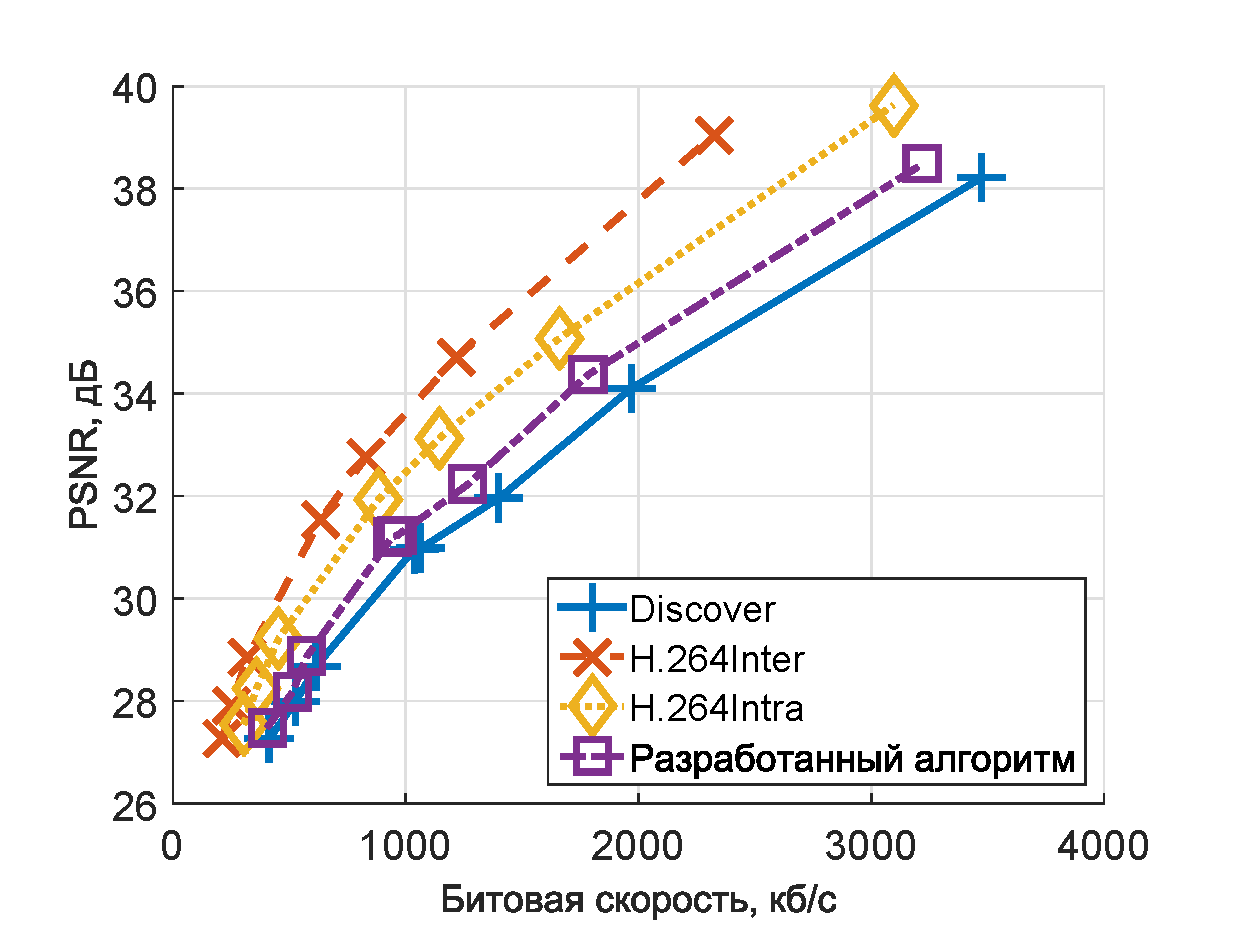
\includegraphics[width=\textwidth]{Chapter4/rdfinal-football-cif-30Hz} \\ Football
        \end{minipage}
    \end{center}
    \caption{Сравнение с существующими алгоритмами сжатия}
    \label{fig:FinalDvcComparisonResults}
\end{figure}

\begin{table}[htbp]
    \begin{center}
        \caption{Результаты сравнения реализованного программного комплекса и кодека DISCOVER по критерию BD-RATE}
        \label{tab:ComparisonWithDiscover}
        \begin{tabular}{|c|c|}
            \hline
            {\bfseries Последовательность } & {\bfseries BD-Rate, \%} \\
            \hline
            Coastguard	& $4.6$		\\
            \hline
            Football	& $12.4$ 	\\
            \hline
            Foreman		& $8.7$		\\
            \hline
            Hall 		& $4.3$		\\
            \hline
            Soccer 		& $15.8$	\\
            \hline
        \end{tabular}
    \end{center}
\end{table}


\section{Выводы по разделу}
\label{chap:ExpResults:Conclusion}

В данном разделе приведены результаты сравнительного анализа разработанных в настоящей диссертационной работе алгоритмов обработки видеоиформации в рамках системы сжатия, основанной на принципах кодирования зависимых источников. Было показано, что в настоящее время не существует открытой реализации распределенного кодека, с помощью которой можно было бы проводить сравнительный анализ различных алгоритмов генерации дополнительной информации декодера и моделирования виртуального канала. В связи с этим, на основе базовой модели распределенного кодирования DISCOVER, была разработана новая программная модель кодека, сравнимая по степени сжатия с кодеком, реализованным в рамках проекта DISCOVER. Были приведены основные особенности данной программной модели, а также решены задачи, связанные с внедрением в данную модель алгоритмов, разработанных в разделах~\ref{chap:SIG} и~\ref{chap:CNM}. Далее была описана методика выполнения сравнительного анализа алгоритмов, в рамках которой были указаны основные особенности, которые необходимо учесть при сравнении. Также, был предложен новый метод сравнительной оценки алгоритмов генерации дополнительной информации декодера, использующий на упрощенную модель кодека без обратной связи. Показано, что разработанные алгоритмы позволяют повысить степень сжатия по сравнению с кодеком DISCOVER на $4-16\%$.

Основные результаты раздела можно сформулировать следующим образом:
\begin{itemize}
    \item разработана программная модель видеокодека, основанная на базовой модели распределенного кодирования Discover;
    \item решены задачи, связанные с внедрением в программную модель алгоритмов, разработанных в разделах~\ref{chap:SIG} и~\ref{chap:CNM};
    \item предложен метод сравнительной оценки алгоритмов генерации дополнительной информации декодера;
    \item продемонстрирован выигрыш от применения алгоритмов, разработанных в настоящей диссертационной работе.
\end{itemize}